%% ----------------------------------------------------------------
%% Thesis.tex -- MAIN FILE (the one that you compile with LaTeX)
%% ---------------------------------------------------------------- 

% Set up the document
\documentclass[a4paper, 11pt, oneside]{Thesis}  % Use the "Thesis" style, based on the ECS Thesis style by Steve Gunn
\graphicspath{{./Figures/}}  % Location of the graphics files (set up for graphics to be in PDF format)
\DeclareGraphicsExtensions{.pdf,.png,.jpg}

% Include any extra LaTeX packages required
\usepackage[square, numbers, comma, sort&compress]{natbib}  % Use the "Natbib" style for the references in the Bibliography
\usepackage{verbatim}  % Needed for the "comment" environment to make LaTeX comments
% \usepackage{vector}  % Allows "\bvec{}" and "\buvec{}" for "blackboard" style bold vectors in maths
\hypersetup{
	urlcolor=black, 
	colorlinks=false,
	allbordercolors={white}
}  % Colours hyperlinks in blue, but this can be distracting if there are many links.

%% ----------------------------------------------------------------
\begin{document}
\frontmatter      % Begin Roman style (i, ii, iii, iv...) page numbering

% Set up the Title Page
\title  {Hoe realiseren we een ontwikkel omgeving waarin niet-programmeurs, zoals 3D artiesten en level designers, efficiënt unieke virtual reality ervaring kunnen creëren in Unreal Engine 4}
\authors  {\texorpdfstring
            {\href{marktarts93@gmail.com}{Mark Arts}}
            {Mark Arts}
            }
\addresses  {\groupname\\\deptname\\\univname}  % Do not change this here, instead these must be set in the "Thesis.cls" file, please look through it instead
\date       {\today}
\subject    {Virtual Reality}
\keywords   {}

\maketitle
%% ----------------------------------------------------------------

\setstretch{1.3}  % It is better to have smaller font and larger line spacing than the other way round

% Define the page headers using the FancyHdr package and set up for one-sided printing
\fancyhead{}  % Clears all page headers and footers
\rhead{\thepage}  % Sets the right side header to show the page number
\lhead{}  % Clears the left side page header

\pagestyle{fancy}  % Finally, use the "fancy" page style to implement the FancyHdr headers

%% ----------------------------------------------------------------
% The "Funny Quote Page"
\pagestyle{empty}  % No headers or footers for the following pages

\null\vfill
% Now comes the "Funny Quote", written in italics
\textit{``I choose a lazy person to do a hard job. Because a lazy person will find an easy way to do it.''}

\begin{flushright}
Bill Gates
\end{flushright}

\vfill\vfill\vfill\vfill\vfill\vfill\null
\clearpage  % Funny Quote page ended, start a new page
%% ----------------------------------------------------------------

% The Abstract Page
\addtotoc{Abstract}  % Add the "Abstract" page entry to the Contents
\abstract{
\addtocontents{toc}{\vspace{1em}}  % Add a gap in the Contents, for aesthetics

The Thesis Abstract is written here (and usually kept to just this page). The page is kept centered vertically so can expand into the blank space above the title too\ldots

}

\clearpage  % Abstract ended, start a new page
%% ----------------------------------------------------------------

\setstretch{1.3}  % Reset the line-spacing to 1.3 for body text (if it has changed)

% The Acknowledgements page, for thanking everyone
% \acknowledgements{
% \addtocontents{toc}{\vspace{1em}}  % Add a gap in the Contents, for aesthetics

% Als eerste wil ik DPI bedanken voor het mogelijk maken en het faciliteren van deze scriptie. Extra dank gaat naar Boy .... die ons met enthousiasme en vertrouwen begeleid heeft.

% Naast DPI ben ik dankbaar voor het zelfde enthousiasme en vertrouwen van Emiel Bakker onze afstudeer begeleider vanuit het HRO.

% Randy Dijkstra, die zijn scriptie aan de andere kant van mijn bureau schreef, wil ik bedanken voor zijn vriendschap. Zonder jou had ik aanzienlijk minder motivatie gehad om een uitdagend onderwerp te kiezen, laat staan het succesvol afronden ervan.

% Als laatste bedank ik mijn ouders voor het dak boven mijn hoofd, mijn avondeten, het wassen, het opruimen en natuurlijk voor alle mogelijkheden die ze mij gegeven hebben om mijzelf te ontwikkelen. 

% }
% \clearpage  % End of the Acknowledgements
%% ----------------------------------------------------------------

\pagestyle{fancy}  %The page style headers have been "empty" all this time, now use the "fancy" headers as defined before to bring them back


%% ----------------------------------------------------------------
\lhead{\emph{Inhoudsopgave}}  % Set the left side page header to "Contents"
\tableofcontents  % Write out the Table of Contents

%% ----------------------------------------------------------------
%\lhead{\emph{List of Figures}}  % Set the left side page header to "List if Figures"
%\listoffigures  % Write out the List of Figures

%% ----------------------------------------------------------------
%\lhead{\emph{List of Tables}}  % Set the left side page header to "List of Tables"
%\listoftables  % Write out the List of Tables

%% ----------------------------------------------------------------
\setstretch{1.5}  % Set the line spacing to 1.5, this makes the following tables easier to read
\clearpage  % Start a new page
 
% Acronym definitions
\newacronym{hro}{HRO}{Hogeschool Rotterdam}
\newacronym{vr}{VR}{Virtual Reality}
\newacronym{vs}{VS}{Visual Scripting}
\newacronym{ue4}{UE4}{Unreal Engine 4}
\newacronym{hud}{HUD}{Head-up Display}

%Print the glossary
\printglossaries

%% ----------------------------------------------------------------
% End of the pre-able, contents and lists of things
% Begin the Dedication page

% \setstretch{1.3}  % Return the line spacing back to 1.3

% \pagestyle{empty}  % Page style needs to be empty for this page
% \dedicatory{Voor all mijn vrienden die om onverklaarbare redenen graag met mij omgaan}

% \addtocontents{toc}{\vspace{2em}}  % Add a gap in the Contents, for aesthetics


%% ----------------------------------------------------------------
\mainmatter	  % Begin normal, numeric (1,2,3...) page numbering
\pagestyle{fancy}  % Return the page headers back to the "fancy" style

% Include the chapters of the thesis, as separate files
% Just uncomment the lines as you write the chapters

%!TEX root = ../Thesis.tex
\chapter{Inleiding}
\lhead{\emph{Inleiding}}

In een periode van 18 weken is er geprobeerd een reeks van basis componenten voor de \gls{ue4} te ontwikkelen waarmee niet-programmeurs efficiënt interactie aan \gls{vr} demo’s kunnen toevoegen.

De \gls{ue4} is gebruikt omdat deze een uitgebreid \gls{vs} systeem heeft die het makkelijk maakt om simpele logica makkelijk uit te drukke, zie hoofdstuk~\ref{ch:visualscripting}. Het \gls{vs} systeem maakt het mogelijk voor niet-programmeurs om simpele logica zelf toe te voegen zonder dat hier een programmeur voor nodig is. Dit zorgt voor een hogere productiviteit en kwaliteit \cite{Cutumisu200732}.

\section{Probleemstelling}

Momenteel is het toevoegen van interactieve elementen in \gls{vr} een intensieve programmeer taak omdat er nog geen interactie standaard is en elke hardware andere input gebruikt. Het is daardoor ook lastig om de geprogrammeerde logica te hergebruiken in een ander project. Hierdoor is er altijd een programmeur nodig om de gewenste functionaliteit toe te voegen of aan te passen. 

In gameontwikkeling zijn er de afgelopen jaren steeds meer technieken ontwikkeld om van deze afhankelijkheid van programmeurs af te komen \cite{Cutumisu200732, ambientbehav}. De oplossing van \gls{ue4} is het gebruikt van Blueprints om interactie in een spel te programmeren. Maar op het moment van schrijven is er nog geen koppeling tussen Blueprints en \gls{vr} interactie.

\section{Doelstelling}

Het creëren van een reeks basis componenten voor \gls{ue4} waarmee niet programmeurs interactieve \gls{vr} demo’s kunnen maken die toegevoegde waarde hebben aan de workflow van DPI.

Aan het eind van dit traject zal het mogelijk zijn om met de gemaakte componenten een bestaande omgeving geschikt te maken voor \gls{vr} en om een nieuwe omgeving op te zetten zonder behulp van een programmeur.

\section{Onderzoeksvraag}

\subsection{Hoofdvraag}

Hoe realiseren we een ontwikkel omgeving waarin niet-programmeurs, zoals 3D modellers en level designers, efficiënt unieke \gls{vr} ervaring kunnen creëren in \gls{ue4}.

\subsection{Deelvragen}

\begin{itemize}  
\item Hoe kan er een koppeling met \gls{vs} gemaakt worden die intuïtief is voor niet programmeurs? 
	\begin{itemize}
	\item Wat is de huidige kennis van computer logica onder de werknemers van DPI?
	\item Is er extra training nodig om met de ontwikkel omgeving aan de slag te gaan?
	\end{itemize}
\item Welke componenten zullen gemaakt moeten worden?
	\begin{itemize}
	\item Wat zijn de huidige taken van een programmeer in het maken van een virtuele omgeving?
	\item Welke tools bestaan er all?
	\item Wat zijn de juiste abstracties van de componenten? 
	\end{itemize}
\item Is het mogelijk de componenten cross-platform te maken?
	\begin{itemize}
	\item Welke platformen zijn relevant?
	\item Wat zijn de verschillende mogelijkheden van deze platformen?
	\end{itemize}
\end{itemize}

\subsection{Onderzoeksmethoden}
\label{subsec:onderzoeksmethoden}

\subsubsection{Hoe kan er een koppeling met Virtual Scripting gemaakt worden die intuïtief is voor niet programmeurs?}

De hoeveelheid abstractie van de componenten zijn afhankelijk van de bestaande intuïtie voor programmeren. Als een gebruiker namelijk snapt hoe de “als dit dan dat” constructie werkt kan er meer vrijheid in de componenten gecreëerd worden.

Als eerst zal er onderzocht moeten worden wat de huidige kennis is van de niet-programmeurs. Dit kan door middel van interviews en een aantal vragen.

Vervolgens zal er onderzocht moeten worden wat een haalbaar moeilijkheidsgraad is en of er baat is van een extra training voor de niet-programmeurs.

Als er sprake is van toegevoegde waarde van een extra training dan zal deze parallel aan het project gegeven worden en iteratief ontwikkeld.

\subsubsection{Welke componenten zullen gemaakt moeten worden?}
Dit zal beginnen met een onderzoek naar de huidige taken vaan programmeur tijdens het maken van een virtuele reality omgeving. Aan de hand hiervan zal er gekeken worden welke taken geautomatiseerd kunnen worden of versimpeld naar \gls{vs}.

Als er een duidelijk beeld is van de benodigde componenten zal er een onderzoek gedaan worden naar bestaande tools die ingezet kunnen worden om de workflow te verbeteren.

Als het duidelijk is welke componenten zelf geschreven moeten worden en hoeverre de niet-programmeurs met \gls{vs} om kunnen gaan kan er bepaald worden welke abstractie de componenten zo breed inzet baar mogelijk houd terwijl het intuïtief blijft voor de niet-programmeurs

\subsubsection{Is het mogelijk de componenten cross-platform te maken?}
Er zal hier onderzocht moeten worden welke platformen relevant zijn en wat de mogelijkheden voor elk platform is.

Er zal daarna een beslissing gemaakt moeten worden voor elk component of het een alternatieve versie moet hebben of dat cross-platform in het component zelf meegenomen kan worden.
 
%!TEX root = ../Thesis.tex
\chapter{Unreal Engine 4}
In dit hoofdstuk word de keuze voor \gls{ue4} uitgelegd en een vergelijking gemaakt met andere engine's.
Ook word een korte introductie gemaakt voor Blueprints.

\section{Waarom de Unreal Engine 4}

Tijdens het kiezen van een Engine waren er drie rand voorwaarden namelijk 
\begin{enumerate}
	\item gratis voor educatie, of goedkoop genoeg voor DPI om aan te schaffen
	\item Oculus en GearVR ondersteuning
	\item Een \gls{vr} systeem
\end{enumerate}

De volgende Engine’s zijn naar gekeken 
\begin{itemize}
\item Unity
\item CRYENGINE
\item Unreal Engine 4
\end{itemize}

\subsection{Unity}

\subsubsection{Licentie}
Unity heeft een educatie licentie waaronder het grootste gedeelte van de engine gratis gebruikt kan worden maar rekening houdend met de interesses van DPI, en eventuele vervolg projecten die zei willen ondernemen, zal de licentie minimaal 75€ per maand worden met daar de koste van Android builds bij.

\subsubsection{Oculus en GearVR ondersteuning}
Van de drie engine’s heeft unity de meest uitgebreide platform support. Daarnaast is Unity vaak een van de eerste keuze’s om nieuwe technieken mee te implementeren. De reden achter deze keuze is het gemak waarop plugins gemaakt kunnen worden en de voordelige / gratis pricing van Unity wat het een populaire keuze maakt voor experimenteren.

\subsubsection{Virtual Scripting}
Unity heeft zelf niet een ingebouwd \gls{vs} systeem maar via een aantal plugins kan dit wel worden toegevoegd. Deze plugins zitten wel vast aan de limitaties van een Unity Plugin. Daarnaast word dit niet officieel gesupporterd door Untiy zelf.

\subsubsection{Gebruiks gemak}
Op gebruiksgemak, in serieuze projecten, fidelity en performance loopt Unity ver achter op de \gls{ue4} en CryEngine. Onderhoudbaar en uitbreidbaarheid van Unity is meestal rampzalig door de manier waarop code voor Unity geschreven word. Vaak is Unity daarom ook niet de keuze voor grote games van hoge kwaliteit. 

Het programmeren word namelijk in een component style in c-sharp gedaan. Het programmeren in c-sharp is voor veel mensen fijn omdat dit vaak een bekende taal is. Maar het component systeem en de manier waarop Unity relatie’s afhandelt zorgt dat er extreem snel spaghetti code ontstaat. 

\subsection{CRYENGINE}
\subsubsection{Licentie}
De CRYENGINE licentie bestaat uit een “Pay what you want” model. Daarnaast beid Crytek een “CRYENGINE Insider Membership“ aan voor 50€ of 150€. 

\subsubsection{Oculus en GearVR ondersteuning}
Op het moment van schrijven ondersteund de CRYENGINE wel de Oculus maar niet de GearVR. Android ondersteuning is mogelijk maar niet officieel ondersteund door Crytek. Dit zal het lastig maken om GearVR te ondersteunen.

\subsubsection{Visual Scripting}
De CRYENGINE heeft een ingebouwd \gls{vs} systeem genaamd Flow. Dit systeem heeft helaas geen ondersteuning voor overerving en de koppeling met c++ bestaat alleen uit het maken van nieuwe nodes en het aanspreken van graphs in c++.

\subsubsection{Gebruiksgemak}
De CryEngine staat bekend als een moeilijke Engine om in te beginnen maar heeft ondertussen bewezen een goede keuze te zijn voor game ontwikkelaars en grotere teams.

Door het gebrek aan persoonlijke ervaring kan ik hier minder over zeggen. Maar door het gebrek aan GearVR ondersteuning is er hier niet meer in verdiept.

\subsection{Unreal Engine 4}
\subsubsection{Licentie}
Het gebruik van de \gls{ue4} is compleet gratis voor educatie en niet-game applicaties zoals architectuur, visualisatie, films etc. Dit betekend dat zowel tijdens het afstuderen als mogelijke vervolg projecten van DPI er geen licentie kosten betaald hoeven te worden.

\subsubsection{Oculus en GearVR ondersteuning}
\gls{ue4} ondersteund zowel de Oculus als Gear VR. Daarnaast ondersteund het ook de meeste randapparatuur voor \gls{vr} zoals Leap Motion en Kinect. Updates hiervoor komen vaak wel later dan voor Unity.
\subsubsection{Visual Scripting}
Unreal heeft een uitgebreid \gls{vs} systeem wat nauw samenwerkt met c++. Alle functies die in c++ beschikbaar zijn zijn beschikbaar via Blueprints. Van elke Blueprint kan ook direct de source code ingesprongen worden, zelfs voor de functies uit de \gls{ue4} libraries.

Het koppelen van c++ aan Blueprints is vrij simpel en ondersteund ook het creëren van events in c++ en functionaliteit hieraan via Blueprints te koppelen.

\subsubsection{Gebruiks gemak}
De leer curve van \gls{ue4} is redelijk stijl maar binnen een paar weken is het mogelijk de belangrijkste te leren. Een punt om rekening mee te houden is dat het zomaar iets maken in de \gls{ue4} vaak verkeerd uitpakt. Daarom is het belangrijk de documentatie, van het onderdeel waar je mee bezig bent, goed te lezen.

Als de basis principes eenmaal onder de knie zijn kan er extreem snel ontwikkeld, en geprototyped, worden met de \gls{ue4} door de implementatie van \gls{vs} en een strakke en goed uitgedachte UI.

\subsubsection{Conclusie}
De CRYENGINE valt af vanwege zijn gebrek aan GearVR support. Dan blijft de keuze over tussen Unity en \gls{ue4}. Untiy heeft een minder style learning curve maar geavanceerde 3D technieken zullen uiteindelijk toch geleerd moeten worden om een hoge kwaliteit te behalen. 

Het visuele scripting systeem van Unity is beperkt en mist de kracht en flexibiliteit die nodig is om deze scriptie succesvol af te ronden. Daar in tegen beid het visuele scripting systeem van \gls{ue4} wel deze mogelijkheden.

\section{Blueprints}
Blueprints is het visuele scripting systeem van \gls{ue4} en wat deze scriptie mogelijk maakt. De beschrijving van Unreal zelf is als volgt:

“Blueprints are special assets that provide an intuitive, node-based interface that can be used to create new types of Actors and script level events; giving designers and gameplay programmers the tools to quickly create and iterate gameplay from within Unreal Editor without ever needing to write a line of code.”

Blueprints ziet er als volgt uit:

\begin{figure}[!ht]
  \centering
    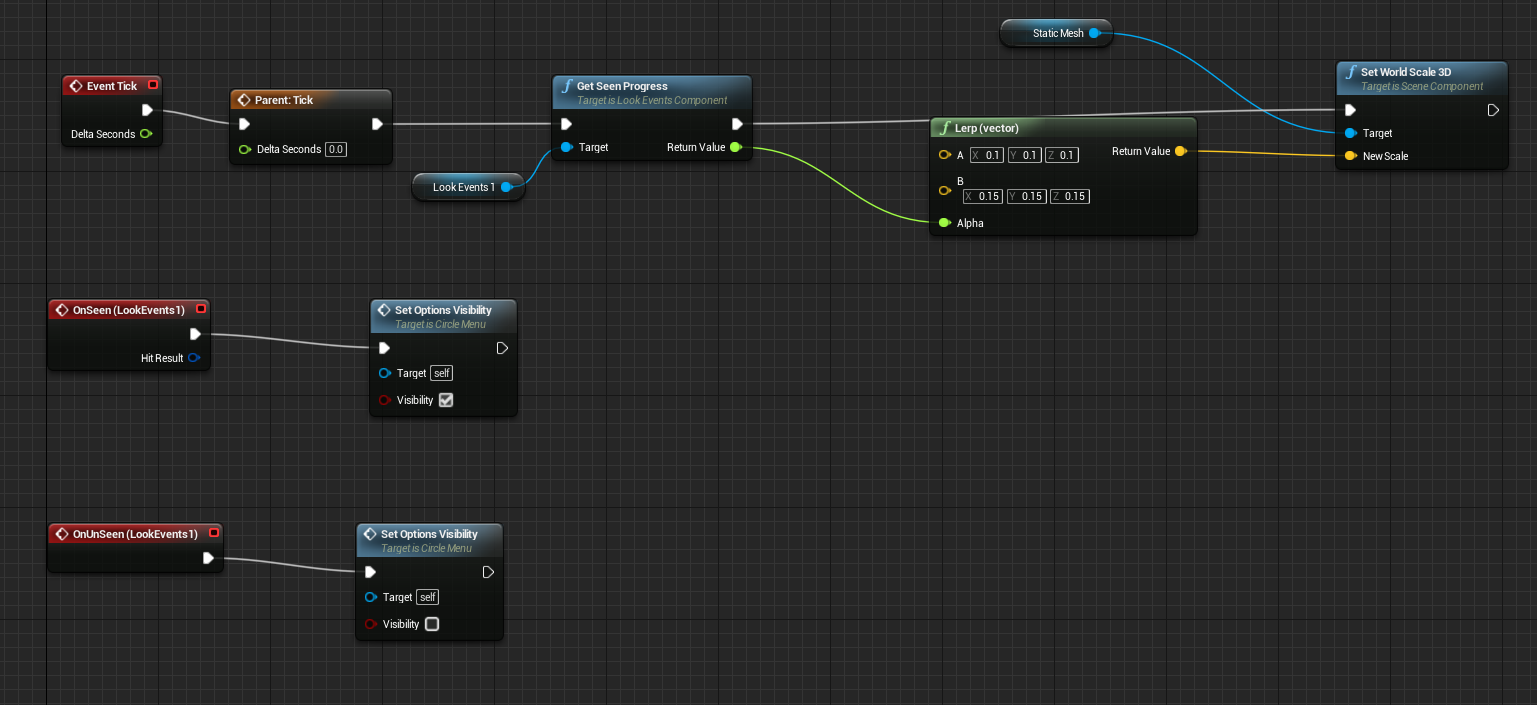
\includegraphics[width=\linewidth,height=\textheight,keepaspectratio]{BluePrintSeenExample}
    \caption{Voorbeeld van een Blueprint.}
\end{figure}

Een hele kort samenvatting zou zijn dat de rode nodes Events zijn en dus aangeven wanneer iets gebeurd, de witte lijnen bepalen de volgorde waarin de nodes worden uitgevoerd, de blauwe nodes zijn functies en de rest zijn variabelen of pure transformatie van data. 
%!TEX root = ../Thesis.tex
\lstset {language=C++}
\lhead{\emph{Visual Scripting}}

\chapter{Visual Scripting}
\label{ch:visualscripting}
In dit hoofdstuk word een introductie gegeven van een visuele programmeer taal. Daarna word er als voorbeeld een vergelijking gemaakt tussen C++ en een visuele taal.

\gls{vs} maakt het mogelijk om logica op een visuele manier in plaats van tekstueel te schrijven. Er is minder kennis van de onderliggende werking van computer systemen nodig dan voor tekstueel programmeren [?]. Hierdoor kan er zonder kennis van computers en hun werking al snel mee gewerkt worden door niet programmeurs. 

\begin{figure}[!ht]
  \centering
    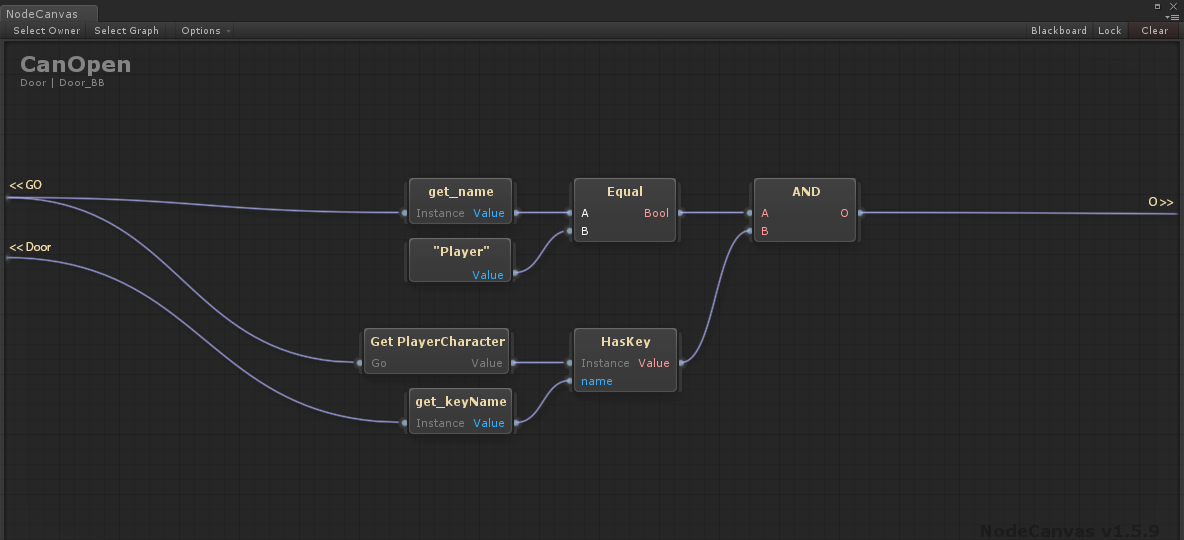
\includegraphics[width=\linewidth,height=\textheight,keepaspectratio]{VisualScriptingExample}
    \caption{Voorbeeld van een visuele script taal.}
\end{figure}

Daarnaast word de mogelijkheden van de visuele programmeer taal ook vaak gelimiteerd om het de gebruiker makkelijker te maken en het programma te beschermen van de gebruiker. Meestal als de limitaties van \gls{vs} een probleem worden had de logica beter in een tekstuele taal geschreven kunnen worden.

\section{Use Case's}
Door de jaren heen zijn er voor verschillende doeleinden visuele programmeer talen gemaakt. 
Een aantal voorbeelden zijn

\begin{itemize}  
\item Data flow in applicaties 
\item State flow voor onder andere animaties 
\item Geluids effecten programmeren
\item Gameplay Logica 
\item Programeren leren aan beginners 
\end{itemize}

In deze scriptie word er gefocust op het gebruik van \gls{vr} voor gameplay logica.

\section{Blueprints}
Blueprints is het visuele scripting systeem van \gls{ue4} en wat deze scriptie mogelijk maakt. De beschrijving van Unreal zelf is als volgt:

“Blueprints are special assets that provide an intuitive, node-based interface that can be used to create new types of Actors and script level events; giving designers and gameplay programmers the tools to quickly create and iterate gameplay from within Unreal Editor without ever needing to write a line of code.”

Blueprints ziet er als volgt uit:

\begin{figure}[H]
  \centering
    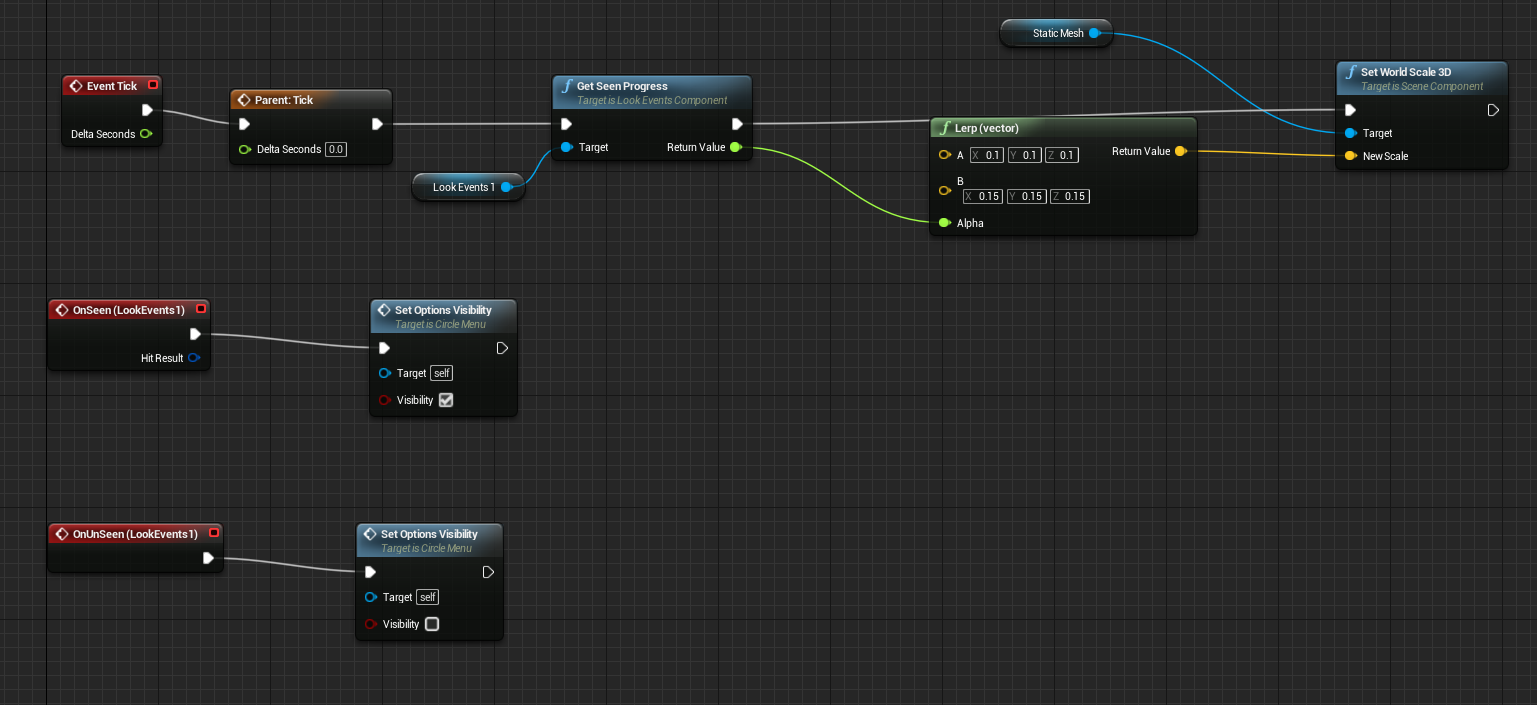
\includegraphics[width=\linewidth,height=\textheight,keepaspectratio]{BluePrintSeenExample}
    \caption{Voorbeeld van een Blueprint.}
\end{figure}

Een hele kort samenvatting zou zijn dat de rode nodes Events zijn en dus aangeven wanneer iets gebeurd, de witte lijnen bepalen de volgorde waarin de nodes worden uitgevoerd, de blauwe nodes zijn functies en de rest zijn variabelen of pure transformatie van data.

\section{Gameplay Logica}
Het programmeren van gameplay in een spel bestaat voor een groot gedeelte uit de vragen “Wanneer moet iets gebeuren”, “Wat moet er gebeuren” en “Hoe moet dit gebeuren”.
De vragen “Waarom moet iets gebeuren” en “Waar moet dit gebeuren” komen het meeste voor in de gameplay logica van een spel, vaak hebben deze vragen ook een makkelijk antwoord. Helaas zijn deze vragen lastig om te beantwoorden in tekstuele code.

\subsection{Het afvuren van een projectiel}
Een voorbeeld van deze drie vragen in code is als volgt, voor het voorbeeld laten wij de logica zien van het schieten van een projectiel in c++ gebaseerd op het standaard voorbeeld van een speler uit de \gls{ue4}.

\subsubsection{Tekstuele Implementatie}
In een c++ header bestand registreren wij de volgende functie in onze speler classe.
\begin{lstlisting}[caption=Registratie van de OnFire functie]
void OnFire();
\end{lstlisting}
Dan tijdens het opzetten van de input voor ons karakter laten we weten wanneer we een projectiel willen schieten.

\begin{lstlisting}[caption=Koppellen van de Fire actie aan de OndFire functie]
if( EnableTouchscreenMovement(InputComponent) == false )
{
	InputComponent->BindAction(
		"Fire", 
		IE_Pressed, 
		this, 
		&Adpi_unreal_colosseumCharacter::OnFire
	);
}
\end{lstlisting}
Maar omdat de “fire” actie niet werkt op een touch interface moeten we de onfire zelf afvuren als iemand het scherm aanraakt (De logica achter het registeren van touch events word niet getoond maar is wel aanwezig in de speler klasse).

\begin{lstlisting}[caption=Aanroepen van de OnFire functie tijdens het EndTouch event]
void Adpi_unreal_colosseumCharacter::EndTouch(const ETouchIndex::Type FingerIndex, const FVector Location)
{
	if (TouchItem.bIsPressed == false)
	{
		return;
	}
	if( ( FingerIndex == TouchItem.FingerIndex ) && (TouchItem.bMoved == false) )
	{
		OnFire();
	}
	TouchItem.bIsPressed = false;
}
\end{lstlisting}
Vervolgens definiëren we OnFire als volgt

\begin{lstlisting}[caption=Implementatie van de OnFire functie]
void Adpi_unreal_colosseumCharacter::OnFire()
{ 
	// try and fire a projectile
	if (ProjectileClass != NULL)
	{
		const FRotator SpawnRotation = GetControlRotation();
		// MuzzleOffset is in camera space, so transform it to world space before offsetting from the character location to find the final muzzle position
		const FVector SpawnLocation = GetActorLocation() + SpawnRotation.RotateVector(GunOffset);

		UWorld* const World = GetWorld();
		if (World != NULL)
		{
			// spawn the projectile at the muzzle
			World->SpawnActor<Adpi_unreal_colosseumProjectile>(ProjectileClass, SpawnLocation, SpawnRotation);
		}
	}

	// try and play the sound and fire animtation if specified
	...

}
\end{lstlisting}
Om de logica te implementeren voor het vuren vuren van de kogel hebben wij nu op vier verschillende plekken de logica moeten verspreiden, hiervan zit de implementatie verspreid in een bestand van 218 regels \ref{appendix:dpi_unreal_colosseumCharacter}.

\subsubsection{Visuele Implementatie}
De “Hoe moet dit gebeuren” is een complexe vraag die prima beantwoord word in code. Vooral omdat er verschillende logica achter elkaar plaatsvind, geluid afspelen / animatie starten, en een aantal wiskundige berekeningen. 

Maar de “Wanneer” vraag is makkelijk te beantwoorden. Namelijk als de fire actie uitgevoerd word of als er op het scherm gedrukt word. De logica in blueprints ziet er als volgt uit (in de event graph van een playerCharacter).

\begin{figure}[!ht]
  \centering
    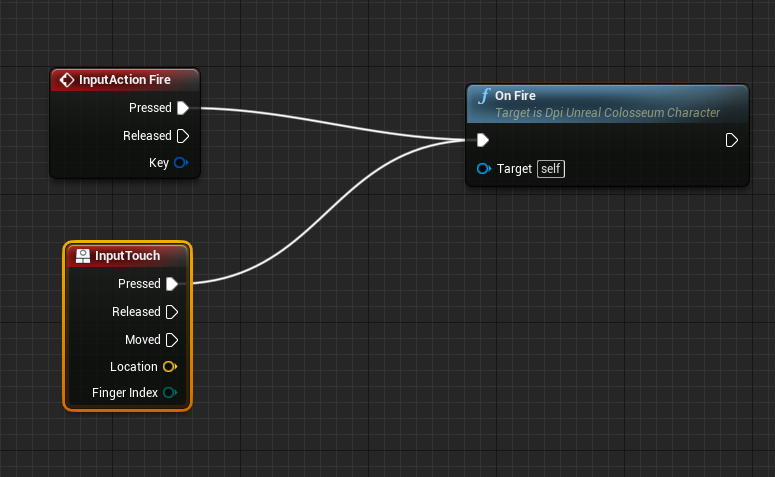
\includegraphics[width=\linewidth,height=\textheight,keepaspectratio]{OnFireBlueprintCall}
    \caption{Afvuren van een projectiel in Blueprints.}
\end{figure}

In tegenstelling tot de c++ code is de logica van de “Wanneer” vraag dit maal niet verspreid en is het in een oog opslag duidelijk wat er voor zorgt dat er een projectiel geschoten word. 
%!TEX root = ../Thesis.tex
\chapter{Uiteenzetting Vooronderzoek}
\label{ch:onderzoek}
\lhead{\emph{Uiteenzetting Vooronderzoek}}

In dit hoofdstuk wordt antwoord gegeven op de volgende vragen door middel van de onderzoeksmethoden beschreven in~\ref{subsec:onderzoeksmethoden}

\begin{itemize}
\item Wat is de huidige kennis van computerlogica onder de werknemers van DPI?
\item Is er extra training nodig om met de ontwikkelomgeving aan de slag te gaan?
\item Welke componenten zullen gemaakt moeten worden?
	\begin{itemize}
	\item Wat zijn de huidige taken van een programmeur bij het maken van een virtuele omgeving?
	\item Welke tools bestaan er al?
	\item Wat zijn de juiste abstracties van de componenten? 
	\end{itemize}
\item Is het mogelijk de componenten cross-platform te maken?
	\begin{itemize}
	\item Welke platformen zijn relevant?
	\item Wat zijn de verschillende mogelijkheden van deze platforms?
	\end{itemize}
\end{itemize}

\section{Wat is de huidige kennis van computerlogica onder de werknemers van DPI?}
Om een idee te krijgen van de huidige kennis van de niet-programmeurs is er begonnen met een enquête over programmeur terminologie \ref{appendix:oreintatieintervieuw:enquete} en een interview over vorige werk ervaringen. \ref{appendix:oreintatieintervieuw:interview}. 

De enquête schept een goed beeld over hoe groot de vorige programmeur-ervaring van de niet-programmeurs is. De correcte terminologie begrijpen van een onderwerp toont namelijk aan dat de er naast het in aanraking met het onderwerp ook bewust kennis is gezocht of gedeeld. En het interview geeft context aan de enquête.

\subsection{Conclusie}
Uit de enquête en het interview blijkt dat er nauwelijks kennis is van programmeren. Wel is er ervaring met 3D software wat het werken in het begin met \gls{ue4} makkelijker zal maken en er sneller gefocust kan worden op het logica aspect.

\section{Is er extra training nodig om met de ontwikkelomgeving aan de slag te gaan?}
Omdat er geen kennis is over het Blueprint systeem van \gls{ue4} of eerder contact is geweest met programmeren, is er besloten om een aantal workshops te geven waarin de niet-programmeurs de basis van Blueprints leren.

\subsection{Conclusie}
In de workshop \ref{appendix:workshop1} is er een introductie gemaakt in de \gls{ue4} en Blueprints. Omdat de niet-programmeurs van een 3D modelling achtergrond komen zijn de verschillen in best practises tussen een game engine en 3d software benadrukt.

In de workshop \ref{appendix:workshop2} krijgen de niet-programmeurs uitleg over Blueprints en de VRInteractions plugin en maken zij zelfstandig een opdracht.

In de workshop \ref{appendix:workshop3} wordt er een complexe opdracht gemaakt en wordt er verwacht dat de niet-programmeurs zelfstandig problemen kunnen oplossen.

\section{Welke componenten zullen gemaakt moeten worden?}
\label{sec:welkeComponenten}
De ontwikkelde componenten zijn gebaseerd op de problemen die de niet-programmeurs tegen komen tijdens het maken en opzetten van \gls{vr} omgevingen. DPI heeft eerder een volledige \gls{vr} ervaring gemaakt in Unity maar deze was niet interactief en gaf weinig input voor het kiezen van componenten. 

Tijdens het schrijven van de scriptie zijn de volgende \gls{vr} omgevingen gemaakt met de VRInteractions plugin

\begin{itemize}
	\item Een fly-trough door een menselijk lichaam
	\item Een appartement waarvan o.a. het meubilair en de vloer dynamisch aangepast kon worden
	\item Een demo van een machine uit een fabriek
	\item Een virtuele omgeving van een tentoonstelling
	\item Een leeromgeving rond het colosseum
	\item Een demo omgeving van de VRInteractions plugin
\end{itemize}

Op basis van de functionaliteit en problemen van deze projecten is de VRInteractions plugin ontwikkeld.

\subsection{Wat zijn de huidige taken van een programmeur in het maken van een Virtuele omgeving?}
DPI focust zich voornamelijk op het maken van exposities in \gls{vr}. Een voorbeeld van een use-case is een opstelling op een beurs vervangen door een \gls{vr} omgeving.

Om de omgeving in te stellen, te starten of tussen omgevingen te navigeren wordt een menu gebruikt waarin de gebruiker opties kan kiezen. Daarnaast wordt er tijdens de demo zelf interactie gebruikt om op een engaging manier informatie te tonen. 

De taken van een programmeur komen in de meeste exposities neer op:

\begin{itemize}
	\item Opzetten van het project
	\item Programmeren van menu en transitie van levels
	\item Programmeren van de triggers voor animaties 
\end{itemize}


\subsection{Welke tools bestaan er al?}
Op het moment van schrijven zijn er een aantal \gls{vr} interactieve producties gemaakt in \gls{ue4}. De producties die het meest lijken op de expositie projecten van DPI zijn:
 
\begin{itemize}
	\item The Rose and I~\footnote{http://store.steampowered.com/app/396060/}
	\item Henry~\footnote{https://storystudio.oculus.com/en-us/henry/}
	\item The Body VR~\footnote{https://www2.oculus.com/experiences/rift/967071646715932/}
\end{itemize}

Deze producties gebruiken voornamelijk het kijken naar elementen als interactie vorm. Maar geen van de projecten heeft bekend gemaakt een toolkit te gebruiken of gesproken over hun implementatie van de interactie.

\subsection{Wat zijn de juiste abstracties van de componenten?}
Blueprints maakt het mogelijk om bepaalde opties te groeperen en als geavanceerd te labelen. 

\begin{figure}[H]
  \centering
    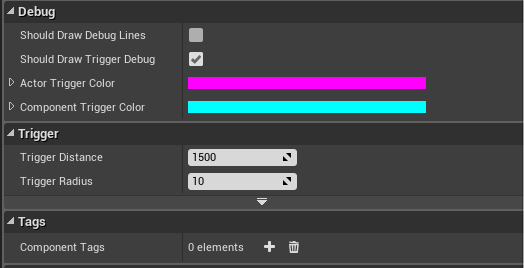
\includegraphics[width=\linewidth/2,height=\textheight/2,keepaspectratio]{Onderzoek_VoorbeeldGeavanceerdDicht}
    \caption{Voorbeeld van de geavanceerde opties die verborgen zijn.}
  \label{fig:advOptiesHidden}    
\end{figure}

\begin{figure}[H]
  \centering
    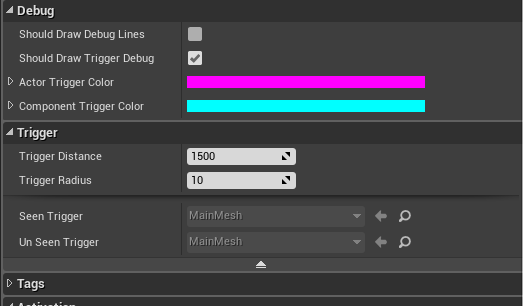
\includegraphics[width=\linewidth/2,height=\textheight/2,keepaspectratio]{Onderzoek_VoorbeeldGeavanceerdOpen}
    \caption{Voorbeeld van de geavanceerde opties die zichtbaar zijn.}
  \label{fig:advOptiesVisible}
\end{figure}

Dit zorgt ervoor dat de componenten zo abstract mogelijk gecodeerd kunnen worden en de opties die voor onduidelijkheid zorgen verborgen kunnen worden. Ook is het mogelijk om versimpelde versies van functies te maken die aanspreekbaar zijn in Blueprints.

\subsection{Conclusie}
Op basis van de gemaakte projecten en de workshops zijn de volgende componenten ontwikkeld voor de VRInteractions plugin:

\begin{itemize}
	\item Een game mode voor een demo waarin de speler kan rondlopen en een voor een fly-through demo
	\item Een speler klasse per game mode
	\item Een component wat verantwoordelijk is voor de input van de speler
	\item Een component wat verantwoordelijk is voor de camera van de speler
	\item Een component die events afvuurt als er naar een object gekeken word
	\item Een HUD die het mogelijk maakt op basis de look events informatie te tonen
	\item Een 3D menu die zijn opties in een cirkel toont
	\item Een object wat verplaats kon worden door middel van ernaar te kijken.
\end{itemize}

Deze zijn in code zo abstract mogelijk opgezet en vervolgens door groepering van de instellingen en het toevoegen van hulp functies versimpelt in Blueprints.

\section{Is het mogelijk de componenten cross-platform te maken?}
De huidige componenten zijn geschreven met het kijken naar objecten als interactie vorm, een interactie vorm die op elk VR device mogelijk is. 

Voor de GearVR, Vive, en de Oculus kan er gebruik gemaakt worden van de camera positie van de speler. Voor \gls{vr} brillen zoals de Cardboard word de positie van de camera niet automatisch gecorrigeerd en moet de headtracking zelf geïmplementeerd worden. 

Voor elke bril die de camera van de speler automatisch update werken de componenten out of the box.

\subsection{Welke platforms zijn relevant?}
\label{subsec:platforms}
De huidige \gls{vr} headsets die in productie zijn, dus niet in een beta fase, zijn de GearVR, Oculus, Vive en de Cardboard. De Oculus en Vive zijn geschikt voor uitgebreide producties van hoge kwaliteit maar de GearVR is gelimiteerd aan de grafische kracht van de gebruikte mobiel, maar werken alleen op een telefoon uit de Samsung Galaxy serie. 

De Cardboard is ook gelimiteerd aan de kracht van de mobiel die gebruikt word maar kan met Android telefoon gebruikt worden. Dit limiteert de grafische mogelijkheden zover dat er geen comfortabele framerate en responsiveness bereikt kan worden.

\subsection{Wat zijn de verschillende mogelijkheden van deze platforms?}
Omdat de controllers van de GearVR, Oculus en de Vive hardware matig van elkaar verschillen is het erg lastig om deze alle drie te ondersteunen. 

De GearVR maakt namelijk gebruik van een touchpad op de bril of een aangesloten gamepad. De Oculus en Vive hebben beiden eigen controllers ontwikkeld maar deze bevatten verschillende knoppen en door het hardware matige verschil moet hier dubbele code voor geschreven worden.

\subsection{conclusie}
Door de interactie te beperken tot het kijken naar objecten is het mogelijk voor de plugin om alle huidige headsets in productie te ondersteunen op de Cardboard gebaseerde headsets na.

Voor dit onderzoek ondersteunen wij daarom alle brillen op de Cardboard na. De GearVR voor de lage instap kosten voor consumenten en portabiliteit en de Oculus en Vive voor hun hogere grafische mogelijkheden.
%!TEX root = ../Thesis.tex
\lstset {language=C++}
% Define block styles
\tikzstyle{decision} = [diamond, draw, fill=blue!20, 
    text width=4.5em, text badly centered, node distance=3cm, inner sep=0pt]
\tikzstyle{block} = [rectangle, draw, fill=blue!20, 
    text width=5em, text centered, rounded corners, minimum height=4em]
\tikzstyle{line} = [draw, -latex']
\tikzstyle{cloud} = [draw, ellipse,fill=red!20, node distance=3cm,
    minimum height=2em]

\chapter{Blueprints en C++}

In dit hoofdstuk word gameplay logica in drie aspecten verdeeld en word voor elk aspect naar de voor en nadelen van C++ en Blueprints gekeken.

Aan de hand van deze vergelijkingen word een workflow gekozen voor het programmeren van deze logica waarin wij het beste uit C++ en Blueprints proberen te combineren.

\section{Gameplay}

Om de scheiding tussen c++ en Blueprints concreet te maken verdelen wij gameplay logica in de volgende vragen:

\begin{itemize}
	\item Wanneer moet iets gebeuren
	\item Wat moet er gebeuren
	\item Hoe moet dit gebeuren
\end{itemize}

Door deze scheiding wordt het makkelijker om de keuze tussen een C++ en een Blueprint implementatie te maken en kunnen er een aantal richtlijnen opgezet worden.

\subsection{Wanneer}
De wanneer vragen zijn vaak makkelijk te beantwoorden, bijvoorbeeld als de speler geraakt word door een projectiel wil ik dat geluid x afgespeeld word, maar moeilijk te coderen door hun asynchrone natuur. Een van de krachtigste voordelen van een Visuele programmeer taal is dat de flow van een programma uitgedrukt kan worden door middel van de lijnen tussen nodes. 

Om het verschil tussen asynchrone logica in C++ en blueprints duidelijk te maken implementeren wij hieronder het afspelen van een geluid nadat een speler dood gaat.

\subsubsection{C++}
We registeren eerst een functie die aangesproken kan worden door de timeout en het geluid wat afgespeeld word in de header van de character.

\begin{lstlisting}	
/** Plays a sound x seconds after the death of the player*/
void AfterDeathSoundTimeOut();

/** Sound to play each time we fire */
UPROPERTY(EditAnywhere, BlueprintReadWrite, Category=Gameplay)
class USoundBase* DeathSound;
\end{lstlisting}

Vervolgens word deze functie geïmplementeerd in de character.cpp

\begin{lstlisting}
void Adpi_unreal_colosseumCharacter::AfterDeathSoundTimeOut() 
{
	UGameplayStatics::PlaySoundAtLocation(this, FireSound, GetActorLocation());
}
\end{lstlisting}

En word de timeout voor het geluid gezet tijdens het doodgaan van de speler.

\begin{lstlisting}
void Adpi_unreal_colosseumCharacter::OnDeath(const FDeathReason Reason)
{
	// death logic
	...

	FTimerHandle UnusedHandler= FTimerHandle();
	GetWorld()->GetTimerManager().SetTimer(
		UnusedHandler, 
		this, 
		&Adpi_unreal_colosseumCharacter::AfterDeathSoundTimeOut, 
		1.0f
	);
}
\end{lstlisting}

We zien hier dat de gerelateerde code op drie verschillende plekken komt te staan, tussen niet relevante code in. Pas na het lezen van de code op deze drie plekken word het duidelijk wat de complete functionaliteit is. Er zijn hier natuurlijk hulpmiddel voor zoals opmerkingen boven code te plaatsen maar bij elke extra taak die, asynchroon, uitgevoerd moet worden word de code complexer en moeilijker te begrijpen. De lezer moet namelijk alle gerelateerde functionaliteit in zijn geheugen hebben.

\subsubsection{Blueprints}
In Blueprints zou deze logica er als volgt uit zien:

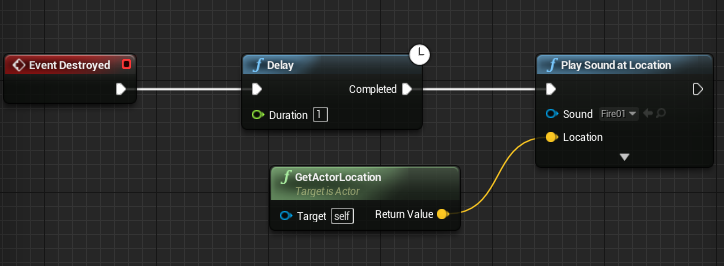
\includegraphics{OnDestroyedSoundDelay}

In de blueprint implementatie is het in een oog opslag duidelijk dat er een geluid afgespeeld word op de locatie van de speler een seconde nadat deze deze dood gaat. De logica bevind zich op de dezelfde plek en de witte lijnen geven de flow van de logica aan. 

Een ander groot verschil dat we hier zien is dat er voor iets simpels als een vertraging in tekstuele code naast de standaard kennis van de c++ syntax ook kennis nodig is van de volgende concepten:

\begin{itemize}
	\item Pointers
	\item Pass by reference
	\item Function references
	\item Namespaces
	\item Out parameters (de UnusedHandler)
	\item Floats
	\item Types
	\item Macros. 
\end{itemize}

Terwijl in Blueprints all deze concepten verborgen zijn in de nodes. Het verbergen van de onderliggende werking van functionaliteit is een thema wat vaker terugkomt in programmeren en wordt aangemoedigd. Het verbergen van deze logica heeft als gevolg dat er zonder programmeer kennis de wanneer logica geïmplementeerd kan worden.

\subsection{Wat}

Het plaatsen van de wat logica in Blueprints of c++ is lastiger om te bepalen. Voor logica die de niet-programmeurs schrijven is c++ geen optie en moet dit wel in Blueprints maar voor programmeurs moet er een afweging gemaakt worden.

Het probleem ontstaat voornamelijk bij complexe conditionele logica.

\subsubsection{Conditionele Logica}

Als we de conditionele logica van het afvuren van de events van een.
LookEventsComponent[zie hoofstuk ?] in c++ en blueprints met elkaar vergelijken.

\begin{itemize}
	\item Bijlage 1: Tick functie van de LookEventsComponent \ref{appendix:LookEventsLogicC}
	\item Bijlage 2: Conditional logic van Tick functie van LookEvents in Blueprints \ref{appendix:LookEventsLogicBlueprints}
\end{itemize}

Zijn beide varianten moeilijk te lezen. Voor iemand die niet codeert ziet de Blueprints variant er waarschijnlijk begrijpgaarder uit maar de complexiteit komt voornamelijk door de logica zelf en in tekstuele code zijn er een aantal manieren om dit soort constructies kleiner te maken zoals:

\begin{lstlisting}
if (bActive != true || (bShouldUsedOnce && TimesUsed > 0) || bIsInTimeOut == true) 
{
	return;
}
\end{lstlisting}
In vergelijking met 

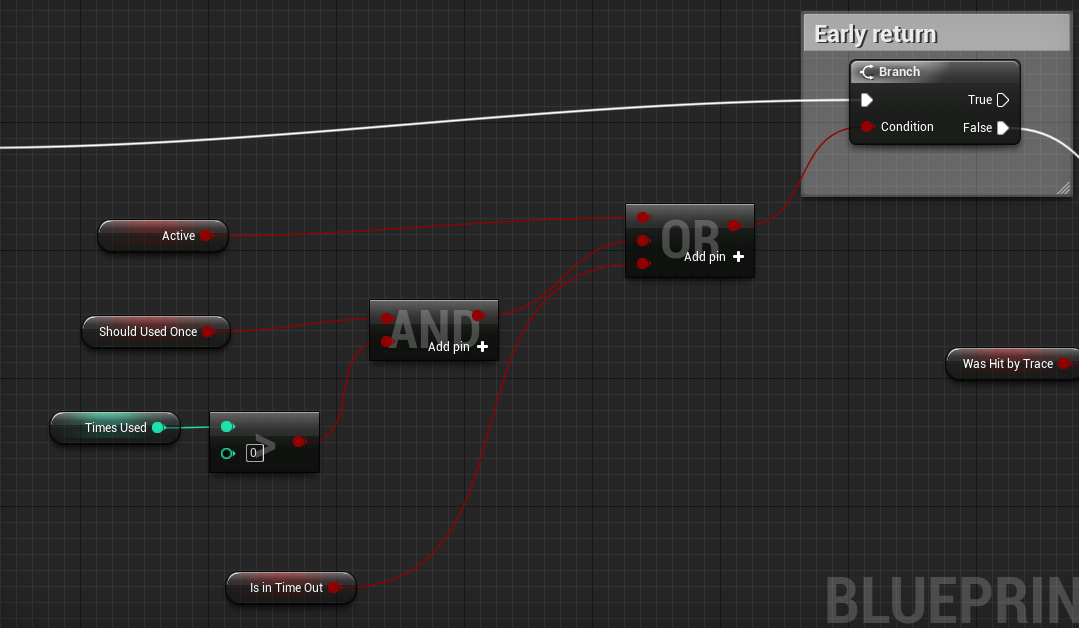
\includegraphics{EarlyReturnBluePrint}

Een ander voorbeeld is de volgende functie die bepaald of de trigger van een LookEventsComponent onderdeel was van een trace.

\begin{lstlisting}
FHitResult ULookEventsComponent::WasHitByTrace(const TArray<FHitResult> HitResults) 
{
	UObject* Trigger = (bIsBeingWatched) ? UnSeenTrigger : SeenTrigger;

	for (auto& HitResult : HitResults)
	{
		UObject* HitObject = (Trigger->IsA(AActor::StaticClass())) ? Cast<UObject>(HitResult.GetActor()) : Cast<UObject>(HitResult.GetComponent());	

		if (HitObject == Trigger)
		{
			if (bShouldDrawTriggerDebug) {
				DebugTrigger(HitObject, 0.1f);
			}
			return HitResult;
		}
	}
	return FHitResult();
}
\end{lstlisting}

In vergelijking met:

\includegraphics{WasHitBytTraceBluePrintExample}

Voor complexe conditionele logica is c++ sneller te begrijpen en geeft meer mogelijkheden om dit te versimpelen. 

\subsection{Hoe}
Met de hoe vraag word de interne werking van een functionaliteit bedoelt waaronder ook de integratie met de rest van het programma, denk aan integratie met de rest van de engine, lifecycles, overerving en performance.

Complexe algoritmes zijn altijd makkelijker in C++ voor zowel leesbaarheid als onderhoudbaarheid. Daarnaast is de scheiding van algoritmes met de rest van de code belangrijk voor het scheiden van complexiteit.

\subsection{Onderhoud en Performance}
Naast het schrijven van de logica zijn performance en onderhoud twee onderwerpen die door elk aspect van een spel verwikkeld zijn en daarom ook onderdeel moeten zijn voor onze keuze van workflow.

\subsubsection{Onderhoud}
Naast een kleine verbetering in leesbaarheid heeft het schrijven van logica in c++ een ander belangrijke voordelen. Namelijk de voordelen van een code editor. Dit geeft uitgebreide debug, zoek en meta informatie. 

De error’s die de Unreal Engine 4 voor je genereed zijn niet altijd even duidelijk, voornamelijk error’s die pas tijdens het packagen van een project ontstaan, en het vinden van een foutieve Blueprint kan extreem lastig zijn. Bijna elk element in de Unreal Engine 4 kan Blueprints code bevatten. En elk element op zich kan die Blueprints weer in kleinere elementen verdelen. Deze elementen bevinden zich tussen alle andere soorten assets zoals Meshes, Animaties, Deciscion Trees, Materials, Textures etc en het zoeken van een onbekende fout hierin is extreem lastig.

Als de foutieve code in c++ had gestaan kan er altijd door middel van een stack trace gekeken worden in welke functie het fout gaat en kan er gezien worden welke functie die functie aansprak en verder omhoog. 

Het auto aan vullen van functie namen en informatie tonen over functies door middel van de JavaDoc opmerking notatie versimpelt het schrijven van complexe code die gebruikt maakt van de Unreal Engine 4. 

\subsubsection{Performance}
Een ander belangrijk onderdeel van de hoe logica is performance. De performance van Blueprints is namelijk lager dan dat van c++. In de hoe en wat vraag is dit verschil compleet onmerkbaar maar in code wat vaak, bijvoorbeeld in de loop van een game, word uitgevoerd kan het verschil merkbaar worden.
In c++ is er ook veel meer controle over de manier waarop de computer logica interpreteert, in Blueprints is dit een stuk minder duidelijk. Dit zorgt ervoor dat op een lager niveau optimalisaties mogelijk zijn. 

Daarnaast is het makkelijker om complexe optimalisaties te schrijven op een onderhoudbaar manier. Als er bijvoorbeeld een performance probleem ontstaat in het aantal raytraces wat de LookEventsComponents nodig hebben is het mogelijk om een cache te schrijven voor de ray traces waar de LookEventsComponent een trace uit vraagt als deze trace dan al eerder door een andere LookEventsComponent berekend is krijg hij de resultaten van die trace inplaats van een nieuwe trace te maken.

\subsection{Conclusie}
Voor de wanneer vraag is Blueprints voor zowel de programmeur als de niet-programmeur altijd de beste optie. Niet alleen is het leesbaarder maar ook flexibeler doordat de logica op een logische manier achter elkaar staat.

Voor de hoe vraag is C++ altijd de beste optie. Onderhoudbaarheid en performance spelen hier een belangrijke rol. 

Voor de wat vraag heeft de niet-programmeur geen optie maar de programmeur wel. Voor triviale code kan er gekozen worden voor Blueprints maar voor complexe conditionele logica heeft C++ de voorkeur. 

\section{Workflow}
Voor onze workflow willen wij de complexiteit voor de niet-programmeurs zo laag mogelijk houden met zo veel mogelijk vrijheid. Daarnaast is flexibiliteit belangrijk voor het makkelijk en veilig experimenteren en itereren.

Gebaseerd op het verdelen van de gameplay logica in de drie vragen hoe, wat en wanneer word er voor de volgende workflow gekozen.
    
\begin{center}
	\begin{tikzpicture}
		[node distance=.8cm,
		start chain=going below,]
			\node[punktchain, join] (Experimenteren) 	
				{Experimenteren (Blueprints)};
			\node[punktchain, join] (hoe)      			
				{Implementatie hoe (C++)};
			\node[punktchain, join] (wat)    			
				{Implementatie complexe wat (C++)};
			\node[punktchain, join] (overerving) 		
				{Blueprints overerving (Blueprints)};
			\node[punktchain, join] (wanneer) 			
				{Wanner en wat (Blueprints)};
	\end{tikzpicture}
\end{center}

Elk component zal beginnen als een imperfecte Blueprint logica. In dit stadium is de performance en onderhoud niet belangrijk, en hoeft het niet eens compleet functioneel te zijn. Er kan direct ge-experimenteert en getest worden. Dit kan niet alleen waardevolle informatie opleveren voor het design aspect van een project maar plaats de logica ook in de context van het project. Vaak komt hier gewenste functionaliteit uit die tijdens het bedenken over het hoofd gekeken is.

Nadat het duidelijk is dat het component gebruikt gaat worden in het project en de gewenste functionaliteiten duidelijk zijn kan er een fatsoenlijke en efficiënte C++ implementatie geschreven worden.

De C++ implementatie word vervolgens overerft door een Blueprint die de aanvullende logica toevoegt.

Ook in gevallen waarin de Blueprint niet iets toe te voegen heeft is het belangrijk om toch een Blueprint te maken van de C++ code. Er kan hierdoor namelijk makkelijk mee geëxperimenteerd worden en niet-programmeurs hebben hierdoor ook de mogelijkheid om iets toe te voegen of een standaard waarde te veranderen.

\section{Versie Controle}
Versie controle is een belangrijk onderdeel van elk ICT project en al valt dit buiten de scope van deze scriptie word er hier een korte vermelding van gemaakt.

Versie controle is een belangrijk onderdeel in samen werken aan code en speelt een belangrijke rol in het onderhoud van code. Er zijn tools in Unreal Engine 4 om versie controle tools zoals git en svn op Blueprints, en assets, toe te passen. Voor deze scriptie is de plugin ontwikkeld met behulp van git maar is er niet gekeken naar een manier waarop niet-programmeurs hier ook mee kunnen werken.

Tijdens de interviews[?] werd het duidelijk dat er geen bestaande kennis van versie controle aanwezig was in de visuele teams van DPI. Het kiezen, opzetten en leren van versie controle en de integratie hiervan met de Unreal Engine 4 valt buiten de scope van deze scriptie.
%!TEX root = ../Thesis.tex
\lstset {language=C++}

\chapter{VRInteractions}
\lhead{\emph{VRInteractions}}
In dit hoofdstuk worden de keuzes voor en de werking van de VRInteractions \gls{ue4} plugin besproken. 
Voor elk component in de plugin word de werking en mogelijkheden getoond. Daarnaast word voor elk component, waar relevant, besproken hoe de workshops de design keuzes beïnvloed heeft.

\section{De plugin}
De VRInteractions plugin is een combinatie van c++ code, Blueprints en overschrijfbare game modes.
De plugin heeft als doel om de \gls{vr} specifieke logica te verbergen voor gameplay logica zodat niet-programmeurs interactieve \gls{vr} omgevingen kunnen maken.

De plugin word ontwikkeld volgens de workflow die beschreven word in Hoofdstuk~\ref{ch:BlueprintsEnCpp} op pagina~\pageref{ch:BlueprintsEnCpp}.

De plugin bevat op moment van schrijven de volgende componenten:
\begin{itemize}
	\item Gamemodes
		\begin{itemize}
			\item VRInteractionsFlyTroughGameMode
			\item VRInteractionsGameMode
		\end{itemize}
	\item Characters
		\begin{itemize}
			\item VRInteractionBaseCharacter
			\item VRInteractionCharacter
			\item VRInteractionsFlyCharacter
		\end{itemize}
	\item VRInteractionsPlayerController
	\item VRInteractionsCameraManager
	\item VRInteractionsHud
	\item LookEventsComponent
	\item CircleMenu
	\item VRMovableMesh
\end{itemize}

\section{Gamemodes}
De plugin bevat de game modes VRInteractionsFlyTroughGameMode en VRInteractionsGameMode. Deze modes zijn beide een uitbreiding van de voorbeeld \gls{ue4} characters. Beide gamemodes zijn geschikt voor zowel de Oculus als de GearVR. 

De game modes zijn bedoelt om de basis instellingen voor \gls{vr} in te stellen en zijn voor de meeste applicaties voldoende. In het geval dat er iets in de gamemode aangepast moet worden is het mogelijk de instelling te overschrijven of de gehele gamemode over te erven.

Omdat er gebruik word gemaakt van een aantal input events is het aan te raden om een project altijd te beginnen als First Person Template.

\subsection{VRInteractionsGameMode}
De VRInteractionsGameMode maakt gebruik van de VRInteractionCharacter, VRInteractionsHud, VRInteractionsPlayerController en de VRInteractionsCameraManager. 

De game mode is bedoeld voor spellen waarin de speler kan rondlopen en zorgt ervoor dat de headset juist word geïnstalleerd en de juiste controllers ingesteld staan.

\subsection{VRInteractionsFlyTroughGameMode}
De VRInteractionsFlyTroughGameMode is een gestripte versie van de VRInteractionsGameMode en maakt gebruik van de VRInteractionsFlyCharacter, VRInteractionsHud, VRInteractionsPlayerController en VRInteractionsCameraManager.

Deze gamemode is bedoelt voor VR projecten waarin de speler door behulp van Matinee rondvliegt.

\section{Characters}
De VRInteractionsCharacters bevatten alle beweging en camera instellingen zoals oog hoogte. De instelling zijn gebaseerd op de \gls{vr} guidelines van Epic \href{https://docs.unrealengine.com/latest/INT/Platforms/VR/ContentSetup/index.html#vrcharactersettings}{https://docs.unrealengine.com/latest/INT/Platforms/VR/ContentSetup/index.html}.
\todo{Fix link styling}


\subsection{VRInteractionBaseCharacter}
De VRInteractionBaseCharacter is de basis voor de VRInteractionCharacter en de VRInteractionsFlyCharacter. Deze character bevat de instellingen voor de camera hoogte en wat \gls{vr} gerelateerde logica zoals het roteren van de speler op basis van zijn kijk richting.

Ook word hierin de GearVR touch pad input afgehandeld.

Het is niet de bedoeling deze classe direct te implementeren. In plaats daarvan kan er gekozen worden voor de VRInteractionCharacter of de VRInteractionsFlyCharacter. Als er een nieuwe soort character gemaakt moet worden kan die natuurlijk overerven van de VRInteractionBaseCharacter.

\subsection{VRInteractionCharacter}
De VRInteractionCharacter is bedoelt voor spellen waarin de speler rond kan lopen. De instellingen en functies zijn op basis van de \gls{ue4} \gls{vr} guidelines en de testen van de \gls{vr} demo gemaakt.

\subsection{VRInteractionsFlyCharacter}
De VRInteractionCharacter is bedoelt voor spellen waarin de speler op een rails loopt. Het is mogelijk deze character makkelijk in Matinee te gebruiken. Verschil met de VRInteractionCharacter, naast het niet registeren van controle gerelateerde input, is dat de camera niet op oog hoogte maar in het midden van de character geplaatst word. Dit maakt het maken van de Matinee sequences logischer.

\section{VRInteractionsPlayerController}
\todo{Add VRInteractionsPlayerController description}

\section{VRInteractionsCameraManager}
\todo{Add VRInteractionsCameraManager description}

\section{VRInteractionsHud}
De VRInteractionsHud is de basis \gls{hud} die een cirkel tekent in het midden van het scherm om aan te geven dat er naar een actor met een LookEvent gekeken word.

\begin{figure}[H]
  \centering
    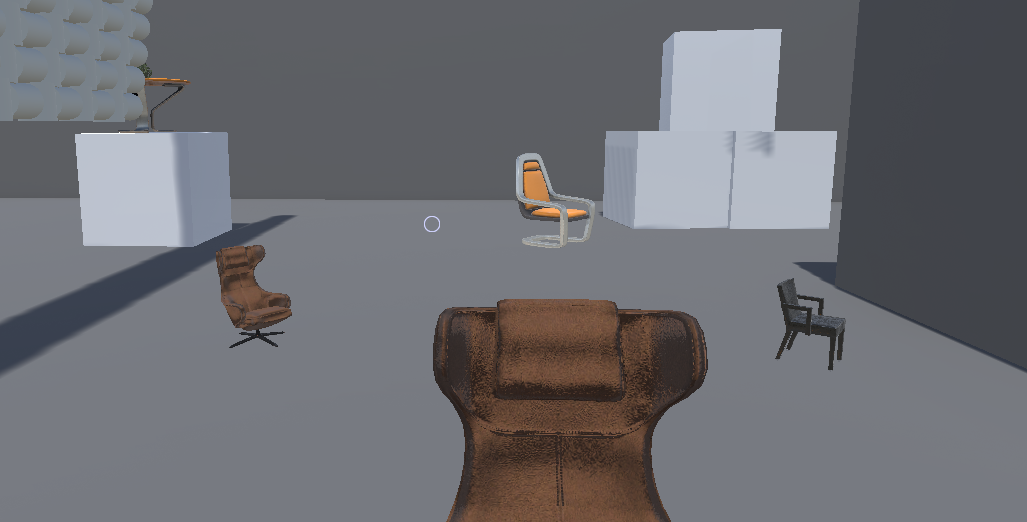
\includegraphics[width=\linewidth,height=\textheight,keepaspectratio]{HudExample}
    \caption{De cirkel die getekend word op het moment dat er naar een Actor met een LookEventsComponent gekeken word.}
\end{figure}

De \gls{hud} is afhankelijk van de VRInteractionsDataSingleton. Om te zorgen dat deze altijd correct word ingeladen kan de singleton als Game Singleton Class ingesteld worden. De singleton word namelijk gebruikt om informatie van de LookEventsComponents te verzamelen.

\section{LookEventsComponent}
De LookEventsComponent vuurt events af op het moment dat er naar de opgegeven trigger gekeken word. Het is mogelijk om meerdere LookEventsComponents aan dezelfde actor toe te voegen waardoor onder andere menu's op basis van kijken gemaakt kunnen worden.

De LookEventsComponent is de basis van de plugin en bijna alle nadere componenten zijn hierop gebaseerd. Interfaces op basis van kijken zijn makkelijk te gebruiken[?] en zijn compatibel met elke \gls{vr} bril.
\todo{Should i source this?}


\subsection{Implementatie}
Voor een aantal weken zijn de LookEvents als zowel een Actor als een Component geïmplementeerd. Het voordeel van een Actor implementatie is dat er vanuit world editor in het rechter muisknop menu event's gekoppeld kunnen worden.

\missingfigure{Screenshot van rechtmuisknop -> add event}

Dit had als nadeel dat het event direct in het level Blueprint gekoppeld word wat aanmoedigt om hier de logica te plaatsen terwijl dit vaak in een Blueprint Actor zou moeten gebeuren.

Ook is het lastig de Actor implementatie binnen een Blueprint Actor te gebruiken, dit kan via een ActorComponent. Het ActorComponent maakt het niet mogelijk om instellingen via de editor te doen en verplicht daardoor om alle settings via Blueprints te zetten, wat omslachtig en fout gevoelig is.

Daarom is er voor de Component implementatie gekozen. Dit maakt het makkelijk om via de Blueprint editor events toe te voegen en kan in combinatie met meerdere LookEvents gebruikt worden. 

\missingfigure{Screenshot van rechtermuis component -> add event}

\subsection{Events}
\todo{Write about how and why the events for LookEvents where implemented}
Om de events zo makkelijk mogelijk te gebruiken is er voor gekozen een

\subsection{Instelling}
De volgende instellingen zijn mogelijk voor de LookEventsComponent:

\begin{itemize}
	\item bShouldUsedOnce
	\item TimesUsed
	\item TriggerTimeOut
	\item SeenDelay
	\item UnSeenDelay
	\item bShouldDrawDebugLines
	\item bShouldDrawTriggerDebug
	\item ActorTriggerColor
	\item ComponentTriggerColor
	\item TriggerDistance
	\item TriggerRadius
	\item bActive
	\item SeenTrigger
	\item UnSeenTrigger
\end{itemize}

\subsubsection{Seen en UnSeen trigger}
De trigger is het object waar naar gekeken kan worden. Er kan voor zowel het triggeren van het Seen event als voor het triggeren van het UnSeen event een ander object gekozen worden.

Er is hier voor gekozen nadat het duidelijk werd dat er vaak een animatie plaatsvind of er extra objecten, bijvoorbeeld een menu, te voor schijn komen die niet in de originele trigger passen.

\begin{figure}[!ht]
  \centering
    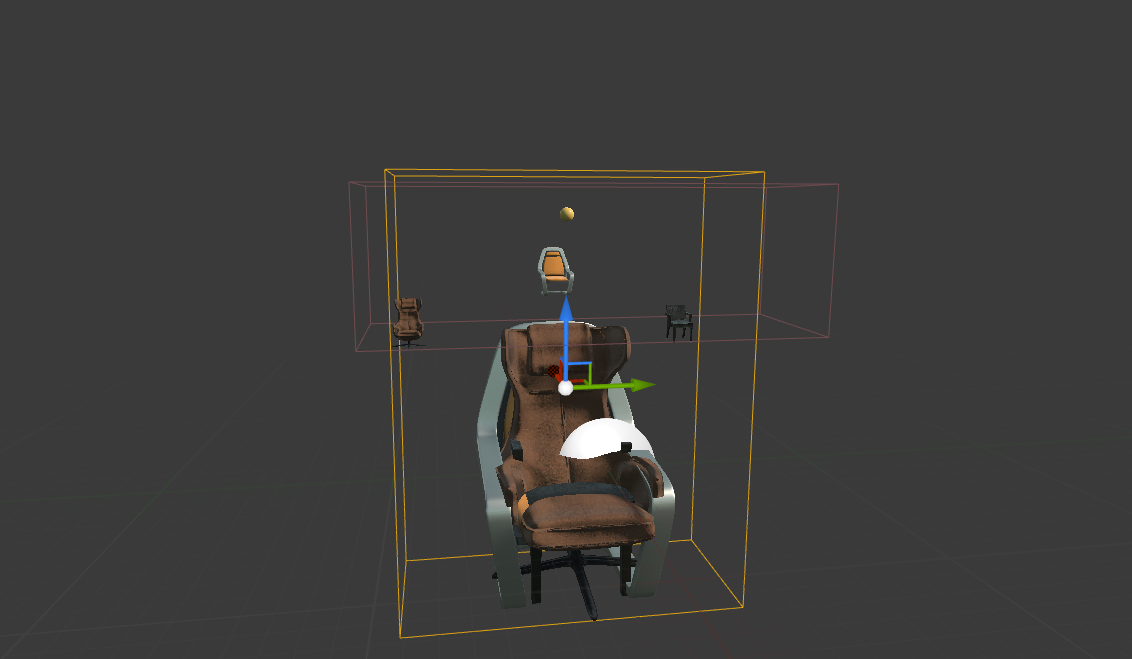
\includegraphics[width=\linewidth,height=\textheight,keepaspectratio]{Voorbeeld_SeenUnseenTriggerBox}
    \caption{Een voorbeeld waarin de geselecteerde trigger box het menu toont en het menu getoond blijft zolang er naar de tweede trigger box gekeken word}
\end{figure}

Als er niet specifiek een trigger opgegeven word word de Actor die het component bevat als Seen en Unseen trigger gezien. De triggers kunnen via blueprint gezet worden.

\begin{figure}[!ht]
  \centering
    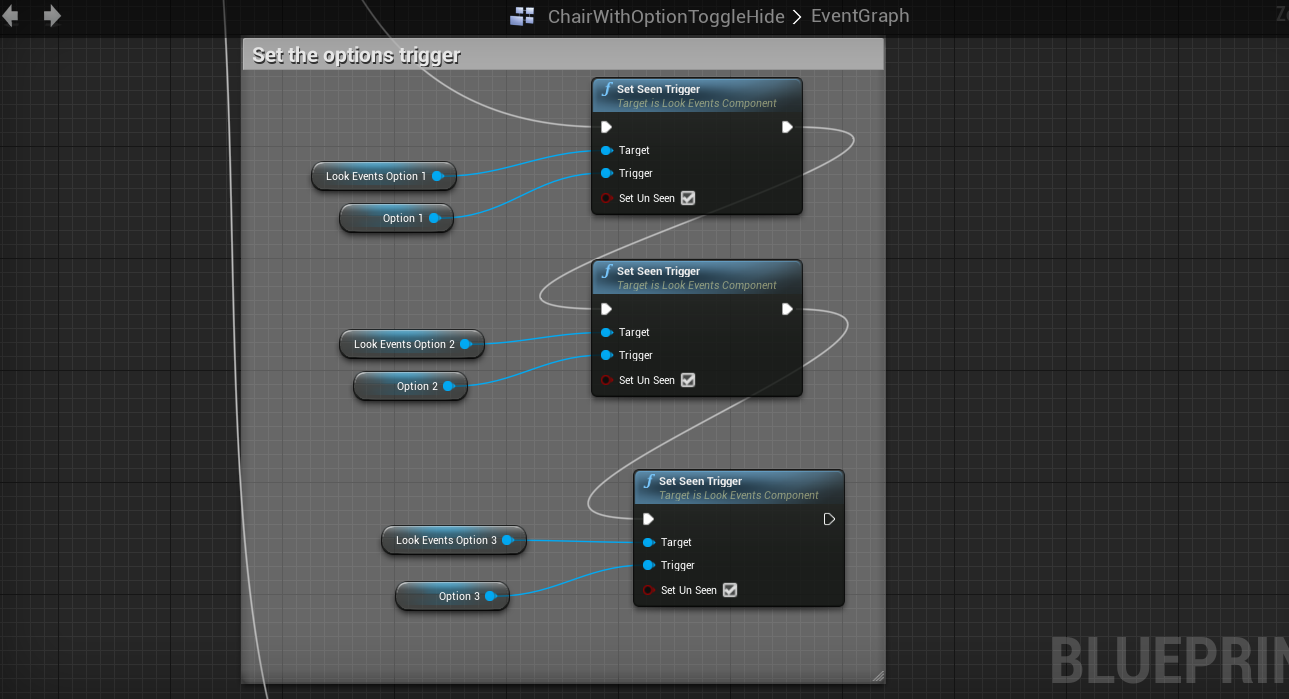
\includegraphics[width=\linewidth,height=\textheight,keepaspectratio]{SetSeenTriggerExample}
    \caption{Een voorbeeld van het instellen van de triggers voor drie verschillende LookEventComponents}
\end{figure}

\subsection{Debugging}
Tijdens de workshops werd er aangegeven dat het lastig was om de LookEvents te debuggen omdat de triggers niet te zien zijn. Er is voor gekozen om dezelfde debugging voor raytraces te implementeren voor de LookEvents.

\begin{figure}[!ht]
  \centering
    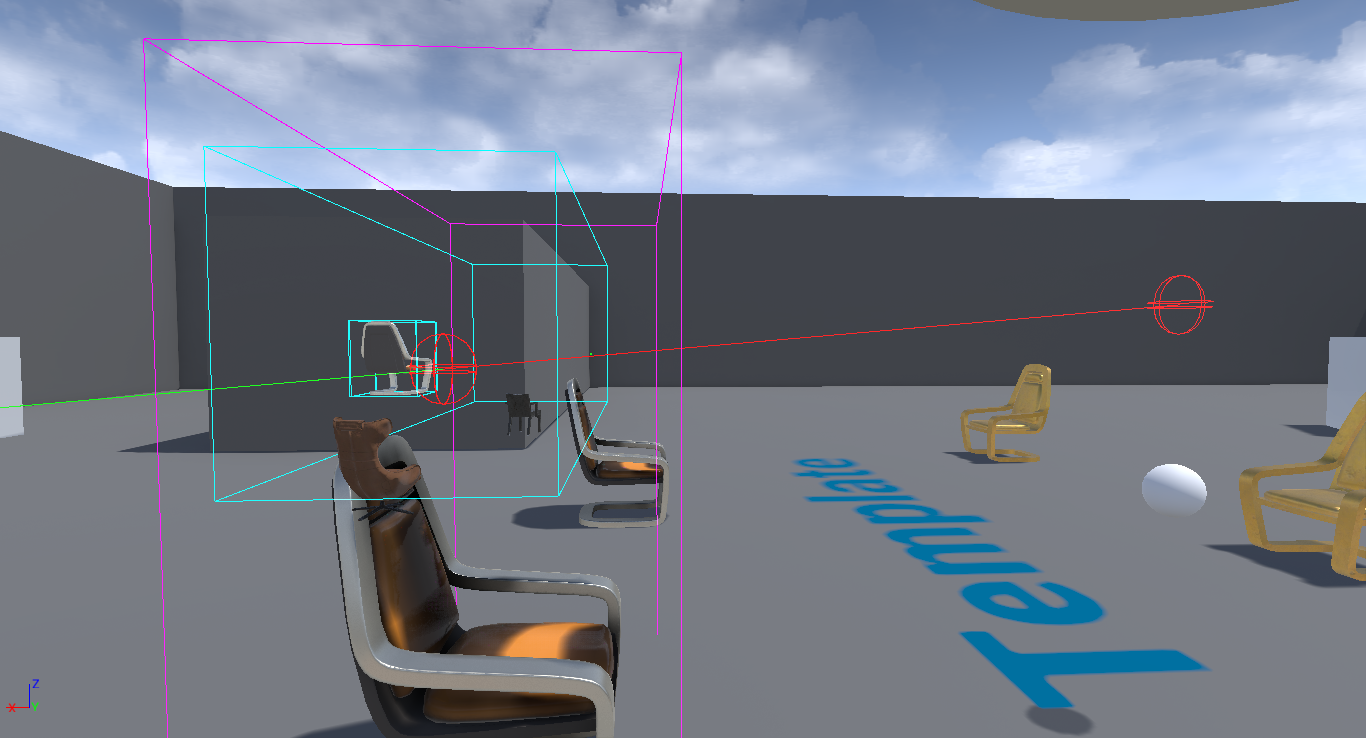
\includegraphics[width=\linewidth,height=\textheight,keepaspectratio]{debugInformatieVanLookEvents}
    \caption{Voorbeeld van debug informatie die een LookEvent kan tekenen.}
\end{figure}

Er word een lijn getekend vanaf de speler ter lengte van de TriggerDistance. Vervolgens word er een vierkant getekend rond de active triggers, er kan een kleur voor Actors en voor Components opgegeven worden. Als er een blocking hit is, door een niet doorzichtig object, word er een cirkel getekend met als diameter de TriggerRadius op de plek waar de blocking hit plaats vond.

\section{CircleMenu}
\dots

\section{VRMovableMesh}
\dots

%\input{Chapters/Chapter5} % Experiment 2

%\input{Chapters/Chapter6} % Results and Discussion

%\input{Chapters/Chapter7} % Conclusion

%% ----------------------------------------------------------------
% Now begin the Appendices, including them as separate files

\addtocontents{toc}{\vspace{2em}} % Add a gap in the Contents, for aesthetics

\appendix % Cue to tell LaTeX that the following 'chapters' are Appendices

%!TEX root = ../Thesis.tex

\chapter{Workshop 1}
\label{appendix:workshop1}
\lhead{}
Deelnemers: Huib, Danny

In de eerste workshop werd een introductie gegeven van Blueprints en \gls{ue4}.
Daarnaast werden de \"best practises\" besproken en een aantal valkuilen tijdens het modellen voor een game engine.

\section{Doel}
\begin{itemize}
	\item Het doornemen van best practises voor UE4 gefocused op verschillen tussen 3D moddeling en 3D games. 
	\item Een begin maken en kennis laten maken met Blueprints.
\end{itemize}

\section{Best practises}
De volgende problemen waren Danny en Huib tegenkomen en werden kort uitgelicht. Er werd ook verteld dat in tegenstelling tot het maken van statische 3D scene het maken van een 3D wereld veel fout gevoeliger is en dat er bewuster met de verschillende elementen van de engine omgegaan moet worden.

De volgende best practises werden toegelicht.
\begin{itemize}
	\item Probeer altijd de documentatie te lezen van een onderdeel voordat je het in productie wilt gebruiken.
	\item Geen scenes in Max maken maar objecten los exporteren en de scene bouwen in \gls{ue4}.
	\item Textures altijd in dimensies in de “Power of Two” maken (4, 8, 16, 32, 64, 128, 256 etc.).
	\item Texture grootte en vertices count zijn belangrijk voor performance in tegenstelling tot 3D moddeling.
	\item Maximale texture grote 4096 * 4096 (2048*2048 voor mobiel).
	\item 65,000 vertices max.
	\item Gebruik altijd het tweede UV channel.
\end{itemize}

Ook werd er gevraagd om de volgende link goed door te lezen als voorbeeld van de \gls{ue4} documentatie
\url{https://docs.unrealengine.com/latest/INT/Engine/Content/FBX/BestPractices/index.html}

\subsection{Ontwikkeling voor mobiel}
De volgende best practises met betrekking tot mobile ontwikkeling werden toegelicht:

\begin{itemize}
	\item Tijdens het opzetten van een project de target hardware setting op mobiel en de quality setting op scalable. 
	\item Het is makkelijker om de kwaliteit te upscalen dan te downscalen.
	\item Voor het mobile platform komen alle assets in de package terecht. Daarom is het belangrijk om niet gebruikte assets te verwijderen.
	\item Maximale texture van 2048*2048 en maximaal 65,000 per object.
	\item De belichting is minder geavanceerd op een mobiel. Daardoor moet er handmatig meer tijd gestopt worden in het zelf belichten van scenes.
\end{itemize}

Ook werd er gevraagd om de volgende link goed door te lezen als voorbeeld van de \gls{ue4} documentatie
\url{https://docs.unrealengine.com/latest/INT/Engine/Content/FBX/BestPractices/index.html}

\section{Workshop}
Na het bespreken van de best practises voor \gls{ue4} werd er voor gedaan hoe een lamp aan en uit gezet kan worden als de speler in de buurt komt door middel van een Blueprint. 

Er werd gevraagd of de lamp ook geleidelijk in sterkte kon toenemen en dit werd ook gedemonstreerd.

\begin{figure}[!ht]
  \centering
    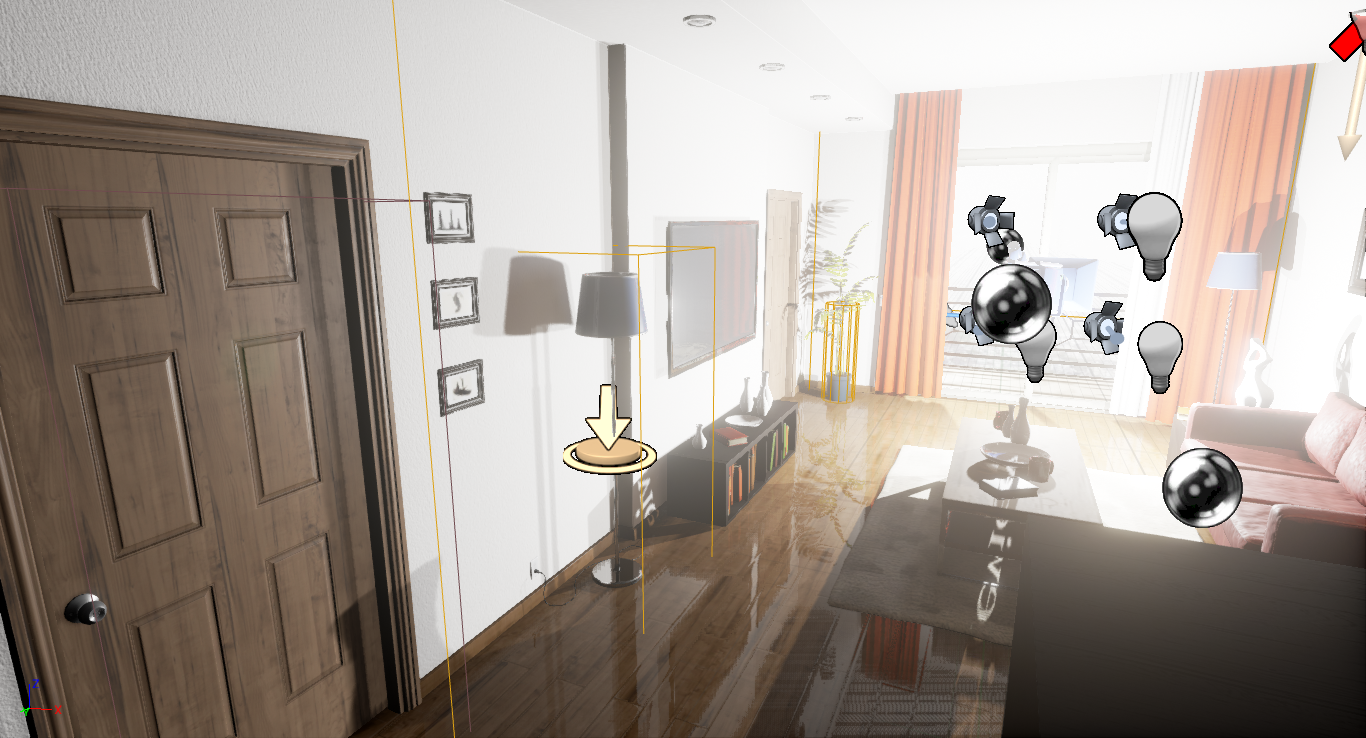
\includegraphics[width=\linewidth,height=\textheight,keepaspectratio]{Workshop_1_lamp}
    \caption{De lamp die aan en uit gezet werd.}
\end{figure}

\begin{figure}[!ht]
  \centering
    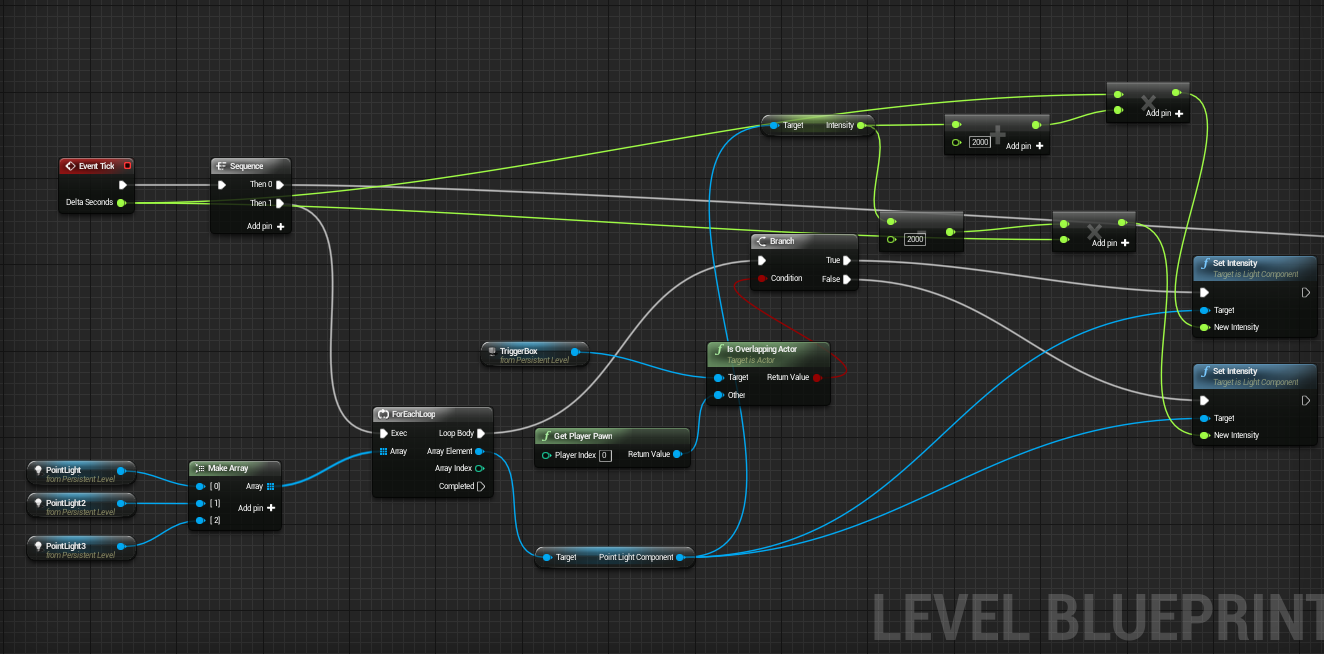
\includegraphics[width=\linewidth,height=\textheight,keepaspectratio]{Workshop_1_LampBlueprint}
    \caption{De Blueprint van het langzaam laten toenemen van de licht sterke van de lamp.}
\end{figure}

\section{Reflectie}
Na de workshop is er met de deelnemers besproken welke van de behandelde onderwerpen onduidelijk waren of interessant om dieper op in te gaan. Op basis hiervan is besloten om dieper op Blueprints, en algemene programmeer logica, in te gaan. Ook is er besloten om in de volgende workshop zelfstandig een opdracht te maken omdat vooral de onderwerpen die het best geleerd kunnen worden door middel van ervaring onduidelijk waren.
%!TEX root = ../Thesis.tex

\chapter{Workshop 2}
\lhead{}
Deelnemers: Danny, Huib

De workshop begon met een uitleg van de concepten die behandeld gaan worden waarna Danny en Huib zelfstandig de opdrachten gingen maken.

Er is voor elke deelnemer een test omgevingen aangemaakt waar de VRInteractions plugin geïnstalleerd is en een aantal voorbeelden bevat die als hulp gebruikt kunnen worden.

\section{Doel}
\begin{itemize}
	\item Kennis laten maken met de VRInteractions plugin en een tv aan en uit zetten door er naar te kijken.
	\item Door de deelnemers zelf te laten programmeren het doel van de komende workshops te bepalen. 
\end{itemize}

\section{Opdrachten}

\subsection{Opdracht 1}
Zet de TV aan door er naar te kijken en pauzeer hem als er niet meer naar gekeken word.

In het oefenproject staat een TV met een promo video van DPI. 
Voeg de LookEvents component aan de TV blueprint toe.
Koppel vervolgens de play en pause van de media texture, het filmpje, aan de Lookevents door middel van de LookEvents component.

\subsection{Opdracht 2}
Zorg dat de LookEvents makkelijker getriggerd worden door een Collisie box te laten bepalen wanneer er naar de TV gekeken word.

Voeg een collison box toe aan de tv blueprint en zet zijn collisie profile op custom en zet alle collisie op ignore behalve de visibility. De visibility moet namelijk op overlap.

Creëer een begin play event en sleep de LookEvents Component in de blueprint. Als je op van de exit node een lijn sleept en los laat kan je in het pop up window zoeken naar “Set Seen Trigger”. Hiermee geef je aan dat je de events wil laten afvuren als naar een specifiek component van de blueprint gekeken word. Zet vervolgens de gemaakt Box Collision als de trigger parameter.

\subsection{Opdacht 3}
Stel de LookEvents in zodat de TV op een kortere (of langere) afstand getriggerd word

Als je de look events component in het components venster (links boven) selecteert verschijnt er aan de rechter kant in het details venster de instelling hiervan. 
Verander de waardes onder de kopjes “User Interaction” en “Trigger” todat jij tevreden bent met het resultaat.

\subsection{Opdracht 4}
Maak een loader die het kijken naar het object duidelijk maakt.

Voeg een statische mesh component toe en zet de statische mesh op de standaard materialshpere.
In de tick functie van de blueprint vraag je de “Seen Progress” van de lookevents door de functie “Get Seen Progress” Op de lookevents component aan te spreken.
Creer nu een “Lerp(Vector”) door met een rechte muisknop in de blueprints het zoek venster te opennen en hierin te zoeken naar de functie.
Zet als waarde A de begin locatie van de Loader en als waarde B zijn eind waarde (waar hij naartoe gaat bewegen)
Vervolgens pak zet je relative locatie  van de loader op de return value van de lerp.

\section{Resultaten}
Uiteindelijk zijn de deelnemers samen de opdracht gaan maken en hebben het volgende ingeleverd:

Yo Mark,

We hebben dit even gezamenlijk gedaan. 

Hier wat onduidelijk heden.

Opdracht 1: we konden in eerste instantie de play node niet vinden.
Het was wat onduidelijk dat we de movie texture moesten verslepen naar media player target.

Opdracht 2 en 3: Event begin play was niet duidelijk. Deze triggerde het filmpje vanaf het begin.
zoals in de afbeelding te zien.

\begin{figure}[!ht]
  \centering
    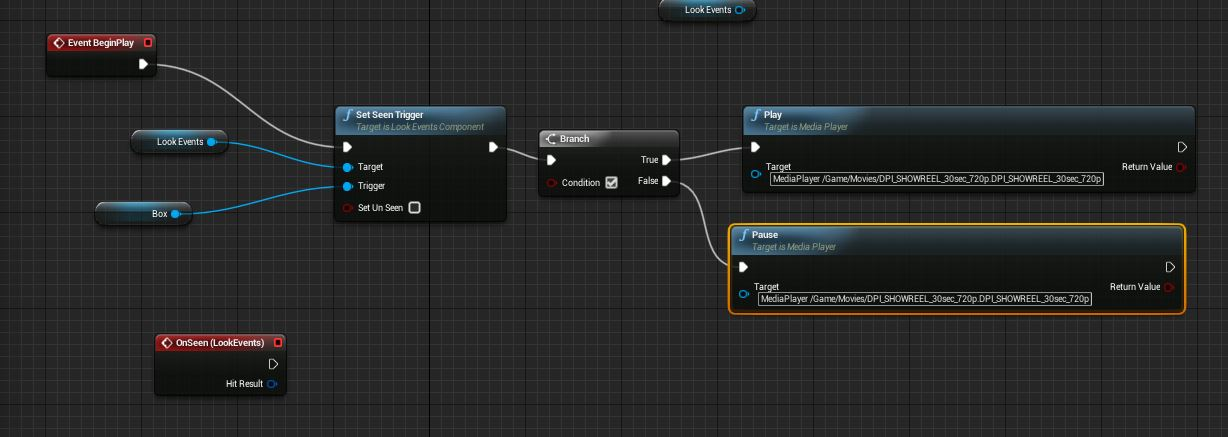
\includegraphics[width=\linewidth,height=\textheight,keepaspectratio]{Workshop_2_Opdracht23_fout}
    \caption{Niet werkende Blueprint van opdracht twee en drie.}
\end{figure}

We probeerde ook wat uit met Branch, maar helaas.

Daarna hebben we weer alles vastgekoppeld aan de OnSeen look event en aan de Event beginPlay. Dit bleek wel te werken.

\begin{figure}[!ht]
  \centering
    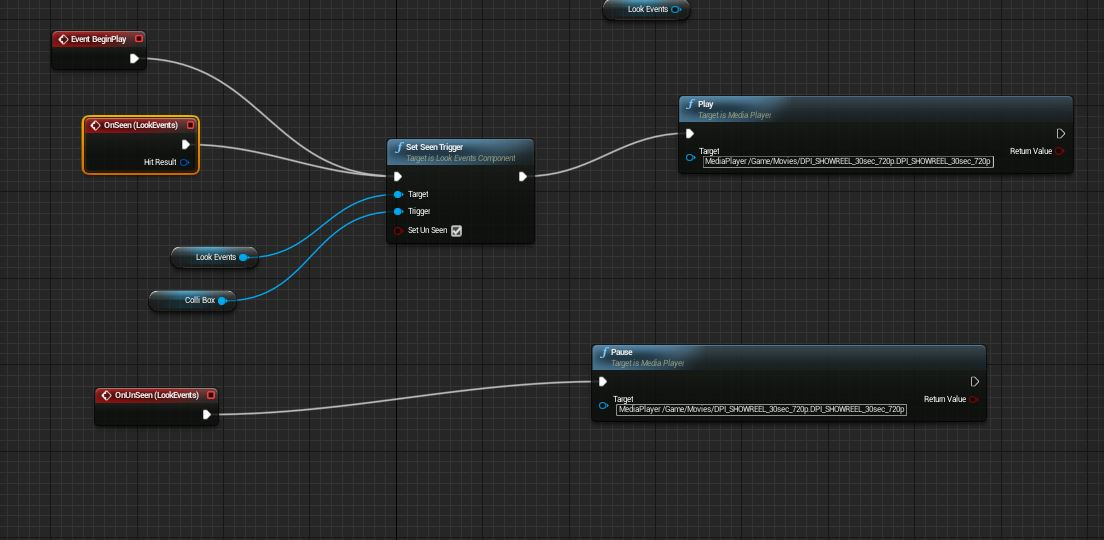
\includegraphics[width=\linewidth,height=\textheight,keepaspectratio]{Workshop_2_Opdracht23_werkend}
    \caption{Functionele Blueprint van opdracht twee en drie.}
\end{figure}


Opdracht4: Uitleg was beter, plaatje werkte ook mee, maar opzich allemaal logisch

\begin{figure}[!ht]
  \centering
    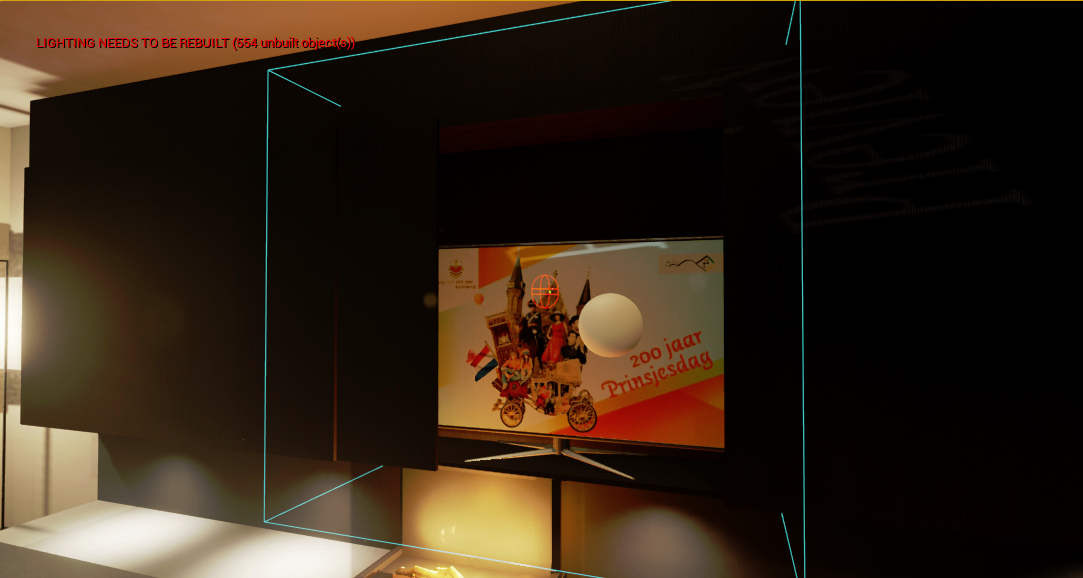
\includegraphics[width=\linewidth,height=\textheight,keepaspectratio]{Workshop_2_eindresultaat}
    \caption{Eind resultaat van de opdrachten.}
\end{figure}

Met Vriendelijke Groet,
Danny Hendriks 

\section{Reflectie}
Het probleem van de play node vinden was inderdaad lastig omdat dit een uitzondering is op hoe de rest van \gls{ue4} werkt. De enige manier om dit soort problemen op te lossen is door ervaring krijgen met hoe de {ue4} werkt.

De uitwerking van opdracht twee en drie was werkend maar het zetten van de LookEvents optie werd in het Tick event gedaan wat voor onverwachte functionaliteit kan zorgen. Dit had eigenlijk tijdens de Begin Play moeten gebeuren.

Na het bespreken van de opdrachten is er gezamenlijk gekozen om de volgende workshops op dezelfde manier aan te pakken, uitleg en dan zelfstandige opdrachten. Ook is er besloten om langzaam dieper in Blueprint scripting te duiken.


%!TEX root = ../Thesis.tex

\chapter{Workshop 3}
\label{appendix:workshop3}
\lhead{}
De workshop begon met een uitleg over de implementatie van de LookEvents uit de VRInteractions plugin en de verschillende configuratie mogelijkheden. Daarnaast is gezamenlijk een vergelijkbare functionaliteit gemaakt zodat het probleem van een node naam niet weten, uit Workshop 2, niet meer voor zou komen.

De workshop is opgenomen en het audio fragment is beschikbaar op aanvraag.

\section{Doel}
Een ingewikkelder versie van de LookEvents implementeren met hierin:

\begin{itemize}
	\item Meerdere look events in een Actor
	\item Veranderden van een material tijdens runtime
	\item Het gebruik en maken van een functie
	\item Het gebruik en maken van variabel
\end{itemize}

\section{Opdrachten}

We gaan een bank maken waar een menu boven zweeft waarmee wij het materiaal van de bank kunnen kiezen. Het menu wordt zichtbaar op het moment dat er naar de bank gekeken wordt.

\subsection{Opdracht 1}
Maak van de bank een Blueprint en voeg hier een scene (dit is een component) aan toe genaamd options met daarin drie static meshes genaamd option0 t/m option2.

Voeg voor elk element een Lookevent component toe en noem die LookEventOption0 t/m LookEventOption2.

\begin{figure}[!ht]
  \centering
    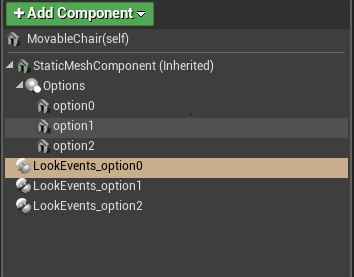
\includegraphics[width=\linewidth,height=\textheight,keepaspectratio]{Workshop_3_AddComponentExample}
    \caption{Voorbeeld van het toevoegen van de LookEvents componenten aan een Actor.}
\end{figure}

Koppel de look events aan de juiste options, kijk hiervoor naar de vorige opdracht, en zet de optie  “Draw debug trigger” aan zodat je makkelijk kan zien of alles werkt.

\subsection{Opdracht 2}
Om te zorgen dat de options alleen zichtbaar worden als er naar de bank gekeken wordt voegen we nog een LookEvents component toe genaamd “LookEventsMain”. 

Om de code schoner te houden maken we een functie genaamd “SetOptionsVisibility” met boolean als input genaamd “Visibility”. In deze functie haal je alle kinderen van de Options scene component op en zet je de visibility hiervan op de input.

\begin{figure}[!ht]
  \centering
    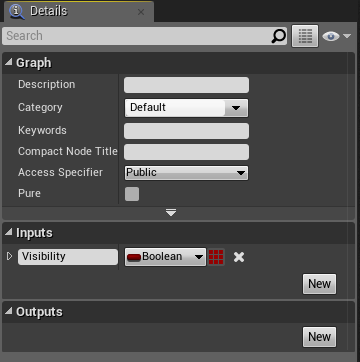
\includegraphics[width=\linewidth,height=\textheight,keepaspectratio]{Workshop_3_functieVoorbeeld}
    \caption{Voorbeeld van een functie in Blueprints.}
\end{figure}

Koppel nu de OnSeen en de OnUnseen events van de “LookEventsMain” aan de “SetOptionsVisibility” functie.

\subsection{Opdracht 3}
We gebruiken de materials van de options static meshes om de material van de bank te bepalen. Op het moment dat er naar een option gekeken wordt (dus het OnSeen event) halen we de material uit de bijhorende option en zetten we material van de hoofd static mesh hierop.

\subsection{Opdracht 4}
Probeer niet de material maar de mesh van de bank te veranderden. Je kan dit doen via de static meshes van de options (zelfde manier als wij de kleuren maken) maar als je een uitdaging wil probeer het via een array variable.

\begin{figure}[!ht]
  \centering
    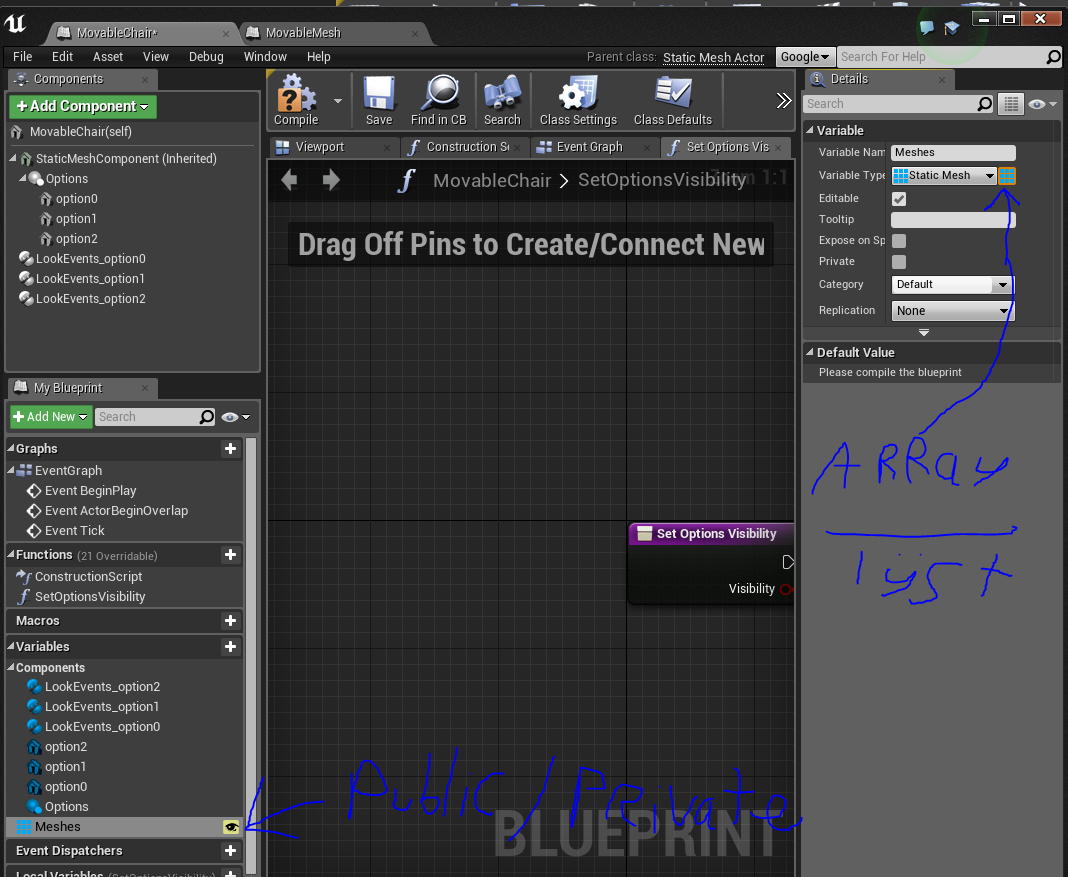
\includegraphics[width=\linewidth,height=\textheight,keepaspectratio]{Workshop_3_variableVoorbeeld}
    \caption{Voorbeeld van een variable in Blueprints.}
\end{figure}

Als je voor een variabel gaat vergeet niet dat dit een lijst van Static Mesh References moet zijn.

\section{Reflectie}
Na het bespreken van de opdracht werd er aangegeven dat er minder tijd kwijt was aan het zoeken naar functienamen omdat een gelijke opdracht van te voren samen gemaakt was. 

Het viel op dat concepten waar in de vorige workshop problemen mee waren dit keer wel goed gingen, bijvoorbeeld het correct zetten van de LookEvents trigger, zonder hier specifieke instructies voor te geven.
%!TEX root = ../Thesis.tex

\chapter{Usability Test 1}
\label{appendix:usertest1}
\lhead{}

Om het gebruiksgemak te meten van de VRInteractions plugin werden de niet-programmeurs gevraagd een probleem op te lossen, waar een optimale oplossing voor is vastgelegd, met behulp van de plugin. 

De gebruikers worden gefilmd tijdens het maken van de opdracht en mogen vragen stellen als ze vast lopen of iets niet begrijpen. De begeleider mag antwoord geven op vragen in een uitleggende vorm maar mag alleen ingrijpen in de opdracht als de niet-programmeur vast zit. De begeleider mag ook ingrijpen als het duidelijk wordt dat de niet-programmeur de opdracht niet begrepen heeft.

Aan de hand van afwijkende stappen en vragen die gesteld moesten worden werd een conclusie getrokken.

\section{De Opdracht}
Voor de opdracht zal er een Mesh generator gemaakt worden. De generator zal bestaan uit een vierkant met hierin een aantal Meshes die als er lang genoeg naar gekeken wordt een MovableMesh versie van zichzelf zullen spawnen.

\subsection{Omschrijving}
Maak een Actor met daarin een triggbox die zichtbaar is tijdens het spelen. In de trigger box plaats je een aantal meshes. Als er naar een mesh gekeken wordt zal deze beginnen met ronddraaien en uiteindelijk zal een MovableMesh versie van de mesh gespawnd worden. 

\subsection{Optimale oplossing}
De volgende stappen zijn de benodigde stappen om tot een optimaal resultaat te komen. Onder het optimaal resultaat valt ook best-practises zoals naamgeving, gebruik van functies en geen vragen.

Maken van de Actor
\begin{itemize}
	\item Maak een nieuwe Actor.
	\item Voeg een trigger box component toe.
		\begin{itemize}
			\item Verander de "Hidden in Game" setting naar false.
		\end{itemize} 
	\item Voeg een sceneComponent toe met een relevante naam (bijvoorbeeld opties).
	\item Voeg een StaticMeshComponent toe voor de gewenste opties.
	\item Voeg een LookEventsComponent toe met een relevante naam (bijvoorbeeld optiesLookEvents).
	\item Maak een functie die alle opties verbergt of toont met een relevante naam (bijvoorbeeld SetOptionsVisibility).
	\item Koppel de OnSeen en OnUnSeen van de optiesLookEvents aan de SetOptionsVisibility.
\end{itemize}

Maken van opties
\begin{itemize}
	\item Voeg een StaticMeshComponent toe aan de opties SceneComponent.
	\item Voeg een LookEventsComponent toe met een relevante naam (bijvoorbeeld ChairLookEvents of Optie1).
	\item Koppel aan de Tick functie de volgende nodes.
		\begin{itemize}
			\item LooKEvents reference
			\item Get Seen Progress
			\item Seen Progress * rotation speed
			\item Add Reltative Rotation to the static mesh
		\end{itemize}
	\item Koppel het OnSeen event aan de volgende nodes
		\begin{itemize}
			\item SpawnActor
			\item SetOptionsVisibility
			\item Delay
			\item SetOptionsVisibility
		\end{itemize}
\end{itemize}

Maken van een MovableMesh variant
\begin{itemize}
	\item Maak een nieuwe Blueprint class.
	\item Kies voor de VRMovableMesh class.
	\item verander de static mesh van de DefaultMesh naar de gewenste Mesh
\end{itemize}

\subsection{Goede oplossing}
Een acceptabel resultaat is een werkende versie van de opdracht zonder bugs of lange termijn performance problemen. Tijdens het maken mogen er geen vragen gesteld worden die een uitleg nodig hebben. Vragen zoals waar kan ik node x vinden zijn toegestaan omdat dit ook in documentatie te vinden is en meer ervaring dan begrip is. 

\subsection{Acceptabele oplossing}
Een acceptabel resultaat is een werkende versie van de opdracht zonder bugs of lange termijn performance problemen. Tijdens het maken mogen er inhoudelijke vragen gesteld worden over werking van de plugin of naar mathematische problemen, zoals het gebruik van lineaire interpolatie.

\subsection{Onacceptabel oplossing}
Als de opdracht niet werkend gekregen wordt zonder het ingrijpen van de begeleider, op onduidelijkheden over de opdracht na.  

\section{Uitvoering}
\dots

\section{Conclusie}
\dots

%!TEX root = ../Thesis.tex
\lstset {language=C++}

\chapter{Implementatie voorbeeld speler Unreal Engine 4}
\label{appendix:dpi_unreal_colosseumCharacter}

\begin{lstlisting}[
	basicstyle=\tiny, 
	caption={dpi unreal colosseumCharacter header}, 
	label={dpiunrealcolosseumCharacterheader}
]
#pragma once
#include "GameFramework/Character.h"
#include "dpi_unreal_colosseumCharacter.generated.h"

class UInputComponent;

UCLASS(config=Game)
class Adpi_unreal_colosseumCharacter : public ACharacter
{
	GENERATED_BODY()

	/** Pawn mesh: 1st person view (arms; seen only by self) */
	UPROPERTY(VisibleDefaultsOnly, Category=Mesh)
	class USkeletalMeshComponent* Mesh1P;

	/** Gun mesh: 1st person view (seen only by self) */
	UPROPERTY(VisibleDefaultsOnly, Category = Mesh)
	class USkeletalMeshComponent* FP_Gun;

	/** First person camera */
	UPROPERTY(VisibleAnywhere, BlueprintReadOnly, Category = Camera, meta = (AllowPrivateAccess = "true"))
	class UCameraComponent* FirstPersonCameraComponent;
public:
	Adpi_unreal_colosseumCharacter();

	/** Base turn rate, in deg/sec. Other scaling may affect final turn rate. */
	UPROPERTY(VisibleAnywhere, BlueprintReadOnly, Category=Camera)
	float BaseTurnRate;

	/** Base look up/down rate, in deg/sec. Other scaling may affect final rate. */
	UPROPERTY(VisibleAnywhere, BlueprintReadOnly, Category=Camera)
	float BaseLookUpRate;

	/** Gun muzzle's offset from the characters location */
	UPROPERTY(EditAnywhere, BlueprintReadWrite, Category=Gameplay)
	FVector GunOffset;

	/** Projectile class to spawn */
	UPROPERTY(EditDefaultsOnly, Category=Projectile)
	TSubclassOf<class Adpi_unreal_colosseumProjectile> ProjectileClass;

	/** Sound to play each time we fire */
	UPROPERTY(EditAnywhere, BlueprintReadWrite, Category=Gameplay)
	class USoundBase* FireSound;

	/** AnimMontage to play each time we fire */
	UPROPERTY(EditAnywhere, BlueprintReadWrite, Category = Gameplay)
	class UAnimMontage* FireAnimation;

protected:
	
	/** Fires a projectile. */
	void OnFire();

	/** Handles moving forward/backward */
	void MoveForward(float Val);

	/** Handles stafing movement, left and right */
	void MoveRight(float Val);

	/**
	 * Called via input to turn at a given rate.
	 * @param Rate	This is a normalized rate, i.e. 1.0 means 100% of desired turn rate
	 */
	void TurnAtRate(float Rate);

	/**
	 * Called via input to turn look up/down at a given rate.
	 * @param Rate	This is a normalized rate, i.e. 1.0 means 100% of desired turn rate
	 */
	void LookUpAtRate(float Rate);

	struct TouchData
	{
		TouchData() { bIsPressed = false;Location=FVector::ZeroVector;}
		bool bIsPressed;
		ETouchIndex::Type FingerIndex;
		FVector Location;
		bool bMoved;
	};
	void BeginTouch(const ETouchIndex::Type FingerIndex, const FVector Location);
	void EndTouch(const ETouchIndex::Type FingerIndex, const FVector Location);
	void TouchUpdate(const ETouchIndex::Type FingerIndex, const FVector Location);
	TouchData	TouchItem;
	
protected:
	// APawn interface
	virtual void SetupPlayerInputComponent(UInputComponent* InputComponent) override;
	// End of APawn interface

	/* 
	 * Configures input for touchscreen devices if there is a valid touch interface for doing so 
	 *
	 * @param	InputComponent	The input component pointer to bind controls to
	 * @returns true if touch controls were enabled.
	 */
	bool EnableTouchscreenMovement(UInputComponent* InputComponent);

public:
	/** Returns Mesh1P subobject **/
	FORCEINLINE class USkeletalMeshComponent* GetMesh1P() const { return Mesh1P; }
	/** Returns FirstPersonCameraComponent subobject **/
	FORCEINLINE class UCameraComponent* GetFirstPersonCameraComponent() const { return FirstPersonCameraComponent; }

};

\end{lstlisting}

\begin{lstlisting}[
	basicstyle=\tiny, 
	caption={dpi unreal colosseumCharacter cpp}, 
	label={dpiunrealcolosseumCharactercpp}
]
#include "dpi_unreal_colosseum.h"
#include "dpi_unreal_colosseumCharacter.h"
#include "dpi_unreal_colosseumProjectile.h"
#include "Animation/AnimInstance.h"
#include "GameFramework/InputSettings.h"

DEFINE_LOG_CATEGORY_STATIC(LogFPChar, Warning, All);

//////////////////////////////////////////////////////////////////////////
// Adpi_unreal_colosseumCharacter

Adpi_unreal_colosseumCharacter::Adpi_unreal_colosseumCharacter()
{
	// Set size for collision capsule
	GetCapsuleComponent()->InitCapsuleSize(42.f, 96.0f);

	// set our turn rates for input
	BaseTurnRate = 45.f;
	BaseLookUpRate = 45.f;

	// Create a CameraComponent	
	FirstPersonCameraComponent = CreateDefaultSubobject<UCameraComponent>(TEXT("FirstPersonCamera"));
	FirstPersonCameraComponent->AttachParent = GetCapsuleComponent();
	FirstPersonCameraComponent->RelativeLocation = FVector(0, 0, 64.f); // Position the camera
	FirstPersonCameraComponent->bUsePawnControlRotation = true;

	// Create a mesh component that will be used when being viewed from a '1st person' view (when controlling this pawn)
	Mesh1P = CreateDefaultSubobject<USkeletalMeshComponent>(TEXT("CharacterMesh1P"));
	Mesh1P->SetOnlyOwnerSee(true);
	Mesh1P->AttachParent = FirstPersonCameraComponent;
	Mesh1P->bCastDynamicShadow = false;
	Mesh1P->CastShadow = false;

	// Create a gun mesh component
	FP_Gun = CreateDefaultSubobject<USkeletalMeshComponent>(TEXT("FP_Gun"));
	FP_Gun->SetOnlyOwnerSee(true);			// only the owning player will see this mesh
	FP_Gun->bCastDynamicShadow = false;
	FP_Gun->CastShadow = false;
	FP_Gun->AttachTo(Mesh1P, TEXT("GripPoint"), EAttachLocation::SnapToTargetIncludingScale, true);


	// Default offset from the character location for projectiles to spawn
	GunOffset = FVector(100.0f, 30.0f, 10.0f);

	// Note: The ProjectileClass and the skeletal mesh/anim blueprints for Mesh1P are set in the
	// derived blueprint asset named MyCharacter (to avoid direct content references in C++)
}

//////////////////////////////////////////////////////////////////////////
// Input

void Adpi_unreal_colosseumCharacter::SetupPlayerInputComponent(class UInputComponent* InputComponent)
{
	// set up gameplay key bindings
	check(InputComponent);

	InputComponent->BindAction("Jump", IE_Pressed, this, &ACharacter::Jump);
	InputComponent->BindAction("Jump", IE_Released, this, &ACharacter::StopJumping);
	
	//InputComponent->BindTouch(EInputEvent::IE_Pressed, this, &Adpi_unreal_colosseumCharacter::TouchStarted);
	if( EnableTouchscreenMovement(InputComponent) == false )
	{
		InputComponent->BindAction("Fire", IE_Pressed, this, &Adpi_unreal_colosseumCharacter::OnFire);
	}
	
	InputComponent->BindAxis("MoveForward", this, &Adpi_unreal_colosseumCharacter::MoveForward);
	InputComponent->BindAxis("MoveRight", this, &Adpi_unreal_colosseumCharacter::MoveRight);
	
	// We have 2 versions of the rotation bindings to handle different kinds of devices differently
	// "turn" handles devices that provide an absolute delta, such as a mouse.
	// "turnrate" is for devices that we choose to treat as a rate of change, such as an analog joystick
	InputComponent->BindAxis("Turn", this, &APawn::AddControllerYawInput);
	InputComponent->BindAxis("TurnRate", this, &Adpi_unreal_colosseumCharacter::TurnAtRate);
	InputComponent->BindAxis("LookUp", this, &APawn::AddControllerPitchInput);
	InputComponent->BindAxis("LookUpRate", this, &Adpi_unreal_colosseumCharacter::LookUpAtRate);
}

void Adpi_unreal_colosseumCharacter::OnFire()
{ 
	// try and fire a projectile
	if (ProjectileClass != NULL)
	{
		const FRotator SpawnRotation = GetControlRotation();
		// MuzzleOffset is in camera space, so transform it to world space before offsetting from the character location to find the final muzzle position
		const FVector SpawnLocation = GetActorLocation() + SpawnRotation.RotateVector(GunOffset);

		UWorld* const World = GetWorld();
		if (World != NULL)
		{
			// spawn the projectile at the muzzle
			World->SpawnActor<Adpi_unreal_colosseumProjectile>(ProjectileClass, SpawnLocation, SpawnRotation);
		}
	}

	// try and play the sound if specified
	if (FireSound != NULL)
	{
		UGameplayStatics::PlaySoundAtLocation(this, FireSound, GetActorLocation());
	}

	// try and play a firing animation if specified
	if(FireAnimation != NULL)
	{
		// Get the animation object for the arms mesh
		UAnimInstance* AnimInstance = Mesh1P->GetAnimInstance();
		if(AnimInstance != NULL)
		{
			AnimInstance->Montage_Play(FireAnimation, 1.f);
		}
	}

}

void Adpi_unreal_colosseumCharacter::BeginTouch(const ETouchIndex::Type FingerIndex, const FVector Location)
{
	if( TouchItem.bIsPressed == true )
	{
		return;
	}
	TouchItem.bIsPressed = true;
	TouchItem.FingerIndex = FingerIndex;
	TouchItem.Location = Location;
	TouchItem.bMoved = false;
}

void Adpi_unreal_colosseumCharacter::EndTouch(const ETouchIndex::Type FingerIndex, const FVector Location)
{
	if (TouchItem.bIsPressed == false)
	{
		return;
	}
	if( ( FingerIndex == TouchItem.FingerIndex ) && (TouchItem.bMoved == false) )
	{
		OnFire();
	}
	TouchItem.bIsPressed = false;
}

void Adpi_unreal_colosseumCharacter::TouchUpdate(const ETouchIndex::Type FingerIndex, const FVector Location)
{
	if ((TouchItem.bIsPressed == true) && ( TouchItem.FingerIndex==FingerIndex))
	{
		if (TouchItem.bIsPressed)
		{
			if (GetWorld() != nullptr)
			{
				UGameViewportClient* ViewportClient = GetWorld()->GetGameViewport();
				if (ViewportClient != nullptr)
				{
					FVector MoveDelta = Location - TouchItem.Location;
					FVector2D ScreenSize;
					ViewportClient->GetViewportSize(ScreenSize);
					FVector2D ScaledDelta = FVector2D( MoveDelta.X, MoveDelta.Y) / ScreenSize;									
					if (ScaledDelta.X != 0.0f)
					{
						TouchItem.bMoved = true;
						float Value = ScaledDelta.X * BaseTurnRate;
						AddControllerYawInput(Value);
					}
					if (ScaledDelta.Y != 0.0f)
					{
						TouchItem.bMoved = true;
						float Value = ScaledDelta.Y* BaseTurnRate;
						AddControllerPitchInput(Value);
					}
					TouchItem.Location = Location;
				}
				TouchItem.Location = Location;
			}
		}
	}
}

void Adpi_unreal_colosseumCharacter::MoveForward(float Value)
{
	if (Value != 0.0f)
	{
		// add movement in that direction
		AddMovementInput(GetActorForwardVector(), Value);
	}
}

void Adpi_unreal_colosseumCharacter::MoveRight(float Value)
{
	if (Value != 0.0f)
	{
		// add movement in that direction
		AddMovementInput(GetActorRightVector(), Value);
	}
}

void Adpi_unreal_colosseumCharacter::TurnAtRate(float Rate)
{
	// calculate delta for this frame from the rate information
	AddControllerYawInput(Rate * BaseTurnRate * GetWorld()->GetDeltaSeconds());
}

void Adpi_unreal_colosseumCharacter::LookUpAtRate(float Rate)
{
	// calculate delta for this frame from the rate information
	AddControllerPitchInput(Rate * BaseLookUpRate * GetWorld()->GetDeltaSeconds());
}

bool Adpi_unreal_colosseumCharacter::EnableTouchscreenMovement(class UInputComponent* InputComponent)
{
	bool bResult = false;
	if(FPlatformMisc::GetUseVirtualJoysticks() || GetDefault<UInputSettings>()->bUseMouseForTouch )
	{
		bResult = true;
		InputComponent->BindTouch(EInputEvent::IE_Pressed, this, &Adpi_unreal_colosseumCharacter::BeginTouch);
		InputComponent->BindTouch(EInputEvent::IE_Released, this, &Adpi_unreal_colosseumCharacter::EndTouch);
		InputComponent->BindTouch(EInputEvent::IE_Repeat, this, &Adpi_unreal_colosseumCharacter::TouchUpdate);
	}
	return bResult;
}

\end{lstlisting}
%!TEX root = ../Thesis.tex
\chapter{Conditional logic van Tick functie van LookEvents in c++}
\lhead{}
\label{appendix:LookEventsLogicC}

\begin{lstlisting}[
	basicstyle=\tiny
]
void ULookEventsComponent::TickComponent(float DeltaTime, enum ELevelTick TickType, FActorComponentTickFunction *ThisTickFunction) 
{

	if (bActive != true || (bShouldUsedOnce && TimesUsed > 0) || bIsInTimeOut == true) 
	{
		return;
	}

	FHitResult HitResult = WasHitByTrace(Trace());

	// TODO: This should be a proppert check if the HitResult was a hit 
	if (HitResult.Actor.IsValid())
	{

		if (bIsInUnSeenDelay) 
		{
			// If we are in a un seen delay we should clear the handler and pretend it never happend
		}

		if (!bIsInSeenDelay) 
		{
			if (SeenDelay > 0 && !bIsSeenDelayFinished) 
			{
			}else if (!bIsBeingWatched) 
			{		
			}
		}
	}
	else if (bIsInSeenDelay)
	{
	}
	else if (bIsBeingWatched) 
	{
		if (UnSeenDelay > 0) 
		{
			if (bIsUnSeenDelayFinished) 
			{				
			}
			else if(!bIsInUnSeenDelay)
			{					
			}
		}else
		{
		}
	}
}
\end{lstlisting}
%!TEX root = ../Thesis.tex
\chapter{Conditional logic van Tick functie van LookEvents in Blueprints}
\lhead{}
\label{appendix:LookEventsLogicBlueprints}
\includegraphics[width=\linewidth,height=\textheight,keepaspectratio]{Figures/WasHitBytTraceBluePrintExample.png}
%!TEX root = ../Thesis.tex

\chapter{Oriëntatie Interview}
\label{appendix:oreintatieintervieuw}
\lhead{}
Interviewer: Mark Arts. Deelnemers: Huib, Danny

\section{Doel}
Het doel van dit interview is om de huidige kennis over gameplay programmering, visuele programmeer talen en logica constructies vast te leggen bij de werknemers van DPI.

Daarnaast wordt er ook een eerst introductie gemaakt naar Blueprints, de visuele programmeer taal die in de Unreal Engine 4 gebruikt wordt.

Er wordt geprobeerd antwoord te krijgen op de volgende vragen:

\begin{itemize}
	\item Welke ervaring met programmeren hebben de deelnemers
	\item Welke ervaring met UE4 hebben de deelnemers
	\item Welke ervaring met visueel programmeren hebben de deelnemers
	\item Tot hoe verre begrijpen de deelnemers programmeer terminologie (enquête)
\end{itemize}

\section{Interview}
\label{appendix:oreintatieintervieuw:interview}
\subsection*{Wat voor 3D projecten hebben jullie tot nu toe gemaakt en wat was jullie taak hierin}
\subsubsection*{Danny}
Voornamelijk het modellen / maken van 3D visualisaties in Max / Maya voor architectuur. Daarnaast een aantal 3D omgevingen in de Unreal Engine 4.
\subsubsection*{Huib}
Voornamelijk het modellen / maken van 3D visualisaties in Max / Maya voor architectuur. Binnen DPI nog niet aan een UE4 project gewerkt. 
\subsection*{Wat is jullie ervaring met Unreal Engine 4}
\subsubsection*{Danny}
Een aantal hobby projecten en binnen DPI het opzetten van een aantal kleine omgevingen in UE4. Lastig om modellen die voor maya / max gebruikt werden te importeren en rekening te houden met performance. De interface van de Engine is wel duidelijk en door ervaring met maya / max was het makkelijk om te beginnen met het bouwen van een omgeving.
\subsubsection*{Huib}
Heeft alleen nog aan hobby projecten gewerkt binnen Unreal maar kon door ervaring met Maya en Max makkelijk aan de slag. Hij had wel moeite met het gebruik van Blueprints in demo’s en vond het vaak overweldigend.
\subsection*{Wat weten jullie over programmeren}
\subsubsection*{Danny}
Geen ervaring met programmeren en weet er weinig over.
\subsubsection*{Huib}
Heeft CMD gestudeerd en heeft tijdens zijn studie ervaring opgedaan met website’s programmeren. Hij snapt hoe code werkt en wat je er mee kan doen maar zou niet C++ voor een game kunnen programmeren.
\subsection*{Wat voor ervaring hebben jullie met visuele programeer talen}
\subsubsection*{Danny}
Geen ervaring.
\subsubsection*{Huib}
Heeft Blueprints geprobeerd maar daarnaast geen ervaring.

\section[Enquête]{Tot hoeverre begrijpen de deelnemers programmeer terminologie (enquête)}
\label{appendix:oreintatieintervieuw:enquete}
Er is door zowel Huib en Danny een vragenlijst ingevuld met de volgende introductie:

Omschrijf in eigen woorden wat jij denkt dat de volgende begrippen betekenen. Als het begrip onbekend is omschrijf wat jij denkt dat het betekent.

\subsection*{Danny}
\textbf{Branch (conditional statement)} \newline
Gok: ik denk een vertakking in verschillende nodes? \newline
\textbf{For loop} \newline
Gok: ik denk een loop in een script, bijvoorbeeld een walkcycle \newline
\textbf{Switch statement} \newline
Gok: True of false switch? \newline
\textbf{Integer} \newline
geen idee \newline
\textbf{Float} \newline
Gok: gravity? geen idee. \newline
\textbf{Boolean} \newline
objecten die met elkaar worden gecombineerd en kan worden bepaald of er gesubstract wordt. \newline
\textbf{Vectors} \newline
De punten van een object (uiteindes) \newline
\textbf{Transform} \newline
Geometry aanpassen in onderandere scalen \newline
\textbf{Struct (structur)} \newline
Gok: hoe een object is opgebouwd? quad en tris? \newline
\textbf{Array} \newline
Op deze manier wordt er iets geduplicate \newline
\textbf{Class} \newline
verschillende blueprints, zoals firstpersonmode of playercontroller. \newline
\textbf{Object Type} \newline
wat voor object, static mesh of een BSP \newline
\textbf{Propertie} \newline
instellingen van bepaalde actors. \newline
\textbf{Reference (pointer)} \newline
Je kan volgens mij objecten converteren naar triggerboxen. \newline
\textbf{Cast} \newline
Gok: ik heb het weleens langs zien komen, maar volgens mij zijn het nodes in het script van Blueprints \newline
\textbf{Actor} \newline
eigenlijk alles wat in de scene wordt gezet. \newline
\textbf{Component} \newline
Gok: heeft iets met de actors te maken, ik denk bepaalde instellingen daarin.

\subsection*{Huib}
\textbf{Branch (conditional statement)} \newline
Keus uit meerdere mogelijkheden / inputs \newline
\textbf{For loop} \newline
Iets doen wanneer iets een bepaalde waarde heeft... \newline
\textbf{Switch statement} \newline
Schakelaar met meer dan 2 mogelijkheden. \newline
\textbf{Integer} \newline
Heel getal \newline
\textbf{Float} \newline
Getal met decimalen \newline
\textbf{Boolean} \newline
True / False \newline
\textbf{Vectors} \newline
Punt in 3D space (x,y,z coördinaat) \newline
\textbf{Transform} \newline
Wat dit in de context van Unreal is weet ik niet, ik ken het als iets dat te maken heeft met de positie, rotatie en schaal van objecten. \newline
\textbf{Struct (structur)} \newline
Constructie van een element. \newline
\textbf{Array} \newline
Een reeks \newline
\textbf{Class} \newline
Een groep objecten met dezelfde eigenschappen. \newline
\textbf{Object Type} \newline
Een soort object, mesh, light, etc. \newline
\textbf{Propertie} \newline
Eigenschap van een object. \newline
\textbf{Reference (pointer)} \newline
Gok: Verwijzing naar iets \newline
\textbf{Cast} \newline
Gok: Iets versturen \newline
\textbf{Actor} \newline
Een object dat ergens op kan reageren. \newline
\textbf{Component} \newline
Een bouwblok

\addtocontents{toc}{\vspace{2em}}  % Add a gap in the Contents, for aesthetics
\backmatter

%% ----------------------------------------------------------------
\label{Bibliography}
\lhead{\emph{Bibliography}}  % Change the left side page header to "Bibliography"
\bibliographystyle{unsrtnat}  % Use the "unsrtnat" BibTeX style for formatting the Bibliography
\nocite{*}
\bibliography{Bibliography}  % The references (bibliography) information are stored in the file named "Bibliography.bib"

\end{document}  % The End
%% ----------------------------------------------------------------